\documentclass[%
%%% PARA ESCOLHER O ESTILO TIRE O SIMBOLO %(COMENTÁRIO)
%SemVinculoColorido,
%SemFormatacaoCapitulo,
%SemFolhaAprovacao,
%SemImagens,
%CitacaoNumerica, %% o padrão é citação tipo autor-data
%PublicacaoDissOuTese, %% (é também o "default") com ficha catal. e folha de aprovação em branco. Caso tenha lista de símbolos e lista de siglas e abreviaturas retirar os comentários dos arquivos siglas.tex e abreviaturasesiglas.tex. Retirar também os comentários indicados nesse arquivo, nos includes
%PublicacaoArtigoOuRelatorio, %% texto sequencial, sem quebra de páginas nem folhas em branco
PublicacaoProposta, %% igual tese/dissertação, mas sem ficha catal. e fol. de aprov.
%PublicacaoLivro, %% com capítulos
%PublicacaoLivro,SemFormatacaoCapitulo, %% sem capítulos
english,portuguese %% para os documentos em Português com abstract.tex em Inglês
%portuguese,english %% para os documentos em Inglês com abstract.tex em Português
,LogoINPE% comentar essa linha para fazer aparecer o logo do Governo
,CCBYNC	% as opções de licença são: CCBY, CCBYSA, CCBYND, CCBYNC, CCBYNCSA, CCBYNCND, GPLv3 e INPECopyright
]{tdiinpe}
%]{../../../../../iconet.com.br/banon/2008/03.25.01.19/doc/tdiinpe}

% PARA EXIBIR EM ARIAL TIRAR O COMENTÁRIO DAS DUAS LINHAS SEGUINTES
%\renewcommand{\rmdefault}{phv} % Arial
%\renewcommand{\sfdefault}{phv} % Arial

% PARA PUBLICAÇÕES EM INGLÊS:
% renomear o arquivo: abnt-alf.bst para abnt-alfportuguese.bst
% renomear o arquivo: abnt-alfenglish.bst para abnt-alf.bst


%%%%%%%%%%%%%%%%%%%%%%%%%%%%%%%%%%%%%%%%%%%%%
%%% Pacotes já previamente carregados:      %
%%%%%%%%%%%%%%%%%%%%%%%%%%%%%%%%%%%%%%%%%%%%%%%%%%%%%%%%%%%%%%%%%%%%%%%%
%%% ifthen,calc,graphicx,color,inputenc,babel,hyphenat,array,setspace, %
%%% bigdelim,multirow,supertabular,tabularx,longtable,lastpage,lscape, %
%%% rotate,caption2,amsmath,amssymb,amsthm,subfigure,tocloft,makeidx,  %
%%% eso-pic,calligra,hyperref,ae,fontenc                               %
%%%%%%%%%%%%%%%%%%%%%%%%%%%%%%%%%%%%%%%%%%%%%%%%%%%%%%%%%%%%%%%%%%%%%%%%
%%% insira neste campo, comandos de LaTeX %%%
%%% \usepackage{_exemplo_}
% etc.
%%%%%%%%%%%%%%%%%%%%%%%%%%%%%%%%%%%%%%%%%%%%%

\watermark{No. 0.1} %% use o comando \watermark para identificar a versão de seu documento
%% comente este comando quando for gerar a versão final
\usepackage{rotating}
\usepackage{dsfont}
\usepackage{comment}
%%%%%%%%%%%%%%%%%%%CAPA%%%%%%%%%%%%%%%%%%%%%%%%%%%%%%%%
%\serieinpe{INPE-NNNNN-TDI/NNNN} %% não mais usado

\titulo{Escrever o título no idioma em que foi escrito a publicação}
\title{Escrever o título em Inglês para publicações escritas em Português e em Português para publicações escritas em Inglês} %% 
\author{Nome Completo do Autor1\\Nome Completo do Autor2} %% coloque o nome do(s) autor(es)
\descriccao{Tese de Doutorado ou Dissertação de Mestrado do Curso de Pós-Graduação em Nome do Curso, orientada pelo(a) Dr(a). Nome do Orientador(a), aprovada em dd de mês por extenso de aaaa.}
\repositorio{aa/bb/cc/dd} %% repositório onde está depositado este documento - na omissão, será preenchido pelo SID
\tipoDaPublicacao{TDI}	%% tipo da publicação (NTC, RPQ, PRP, MAN, PUD, TDI, TAE e PRE) na ausência do número de série INPE, caso contrário deixar vazio
\IBI{xx/yy} %% IBI (exemplo: J8LNKAN8PW/36CT2G2) quando existir, caso contrário o nome do repositório onde está depositado o documento

\date{AAAA}%ano da publicação

%%%%%%%%%%%%%%%%%%%%%%%%%%VERSO DA CAPA%%%%%%%%%%%%%%%%%%%%%%%%%%%%%%%%%%%%%%%%%%%%%%%
\tituloverso{\vspace{-0.9cm}\textbf{\PublicadoPor:}}
\descriccaoverso{Instituto Nacional de Pesquisas Espaciais - INPE\\
Gabinete do Diretor (GB)\\
Serviço de Informação e Documentação (SID)\\
Caixa Postal 515 - CEP 12.245-970\\
São José dos Campos - SP - Brasil\\
Tel.:(012) 3945-6923/6921\\
Fax: (012) 3945-6919\\
E-mail: {\url{pubtc@sid.inpe.br}}
}

\descriccaoversoA{\textbf{\ConselhoDeEditoracao:}\\
\textbf{\Presidente:}\\
Marciana Leite Ribeiro - Serviço de Informação e Documentação (SID)\\
\textbf{\Membros:}\\
Dr. Gerald Jean Francis Banon - Coordenação Observação da Terra (OBT)\\
Dr. Amauri Silva Montes - Coordenação Engenharia e Tecnologia Espaciais (ETE)\\
Dr. André de Castro Milone - Coordenação Ciências Espaciais e Atmosféricas (CEA)\\
Dr. Joaquim José Barroso de Castro -  Centro de Tecnologias Espaciais (CTE)\\
Dr. Manoel Alonso Gan - Centro de Previsão de Tempo e Estudos Climáticos (CPT)\\
Drª Maria do Carmo de Andrade Nono - Conselho de Pós-Graduação\\
Dr. Plínio Carlos Alvalá - Centro de Ciência do Sistema Terrestre (CST)\\
\textbf{\BibliotecaDigital:}\\
Dr. Gerald Jean Francis Banon - Coordenação de Observação da Terra (OBT)\\
Clayton Martins Pereira - Serviço de Informação e Documentação (SID)\\
%Jefferson Andrade Ancelmo - Serviço de Informação e Documentação (SID)\\
%Simone A. Del-Ducca Barbedo - Serviço de Informação e Documentação (SID)\\
%Deicy Farabello - Centro de Previsão de Tempo  e Estudos Climáticos (CPT)\\
\textbf{\RevisaoNormalizacaoDocumentaria:}\\
Simone Angélica Del Ducca Barbedo - Serviço de Informação e Documentação (SID) \\
%Marilúcia Santos Melo Cid - Serviço de Informação e Documentação (SID)\\
Yolanda Ribeiro da Silva Souza - Serviço de Informação e Documentação (SID)\\
\textbf{\EditoracaoEletronica:}\\
Marcelo de Castro Pazos - Serviço de Informação e Documentação (SID)\\
André Luis Dias Fernandes - Serviço de Informação e Documentação (SID)\\
}

%%%%%%%%%%%%%%%%%%%FOLHA DE ROSTO

%%%%%%%%%%%%%%%FICHA CATALOGRÁFICA
%% NÃO PREENCHER - SERÁ PREENCHIDO PELO SID

\cutterFICHAC{Cutter}
\autorUltimoNomeFICHAC{Sobrenome, Nomes} %% exemplo: Fuckner, Marcus André
\autorFICHAC {Nome Completo do Autor1; Nome Completo do Autor2} %% Campo opcional (se não usado prevalece \author)
\tituloFICHAC{Titulo da publicação}
\instituicaosigla{INPE}
\instituicaocidade{São José dos Campos}
\paginasFICHAC{\pageref{numeroDePáginasDoPretexto} + \pageref{LastPage}} %% número total de páginas
%\serieinpe{INPE-00000-TDI/0000} %% não mais usado
\palavraschaveFICHAC{1.~Palavra chave. 2.~Palavra chave 3.~Palavra chave. 4.~Palavra chave. 5.~Palavra chave  I.~\mbox{Título}.} %% recomenda-se pelo menos 5 palavras-chaves - \mbox{} é para evitar hifenização 
\numeroCDUFICHAC{000.000} %% número do CDU 

% Nota da ficha (para TD)
\tipoTD{Dissertação ou Tese} % Dissertação ou Tese
\cursoFA{Mestrado ou Doutorado em Nome do Curso}
\instituicaoDefesa{Instituto Nacional de Pesquisas Espaciais}
\anoDefesa{AAAA} % ano de defesa 
\nomeAtributoOrientadorFICHAC{Orientador}	% pode ser: Orientador, Orientadora ou Orientadores
\valorAtributoOrientadorFICHAC{José da Silva} % nome(s) completo(s)

%%%%%%%%%%%%%%%FOLHA DE APROVAÇAO PELA BANCA EXAMINADORA
\tituloFA{\textbf{ATENÇÃO! A FOLHA DE APROVAÇÃO SERÁ INCLUIDA POSTERIORMENTE.}}
%\cursoFA{\textbf{}}
\candidatoOUcandidataFA{}
\dataAprovacaoFA{}
\membroA{}{}{}
\membroB{}{}{}
\membroC{}{}{}
\membroD{}{}{}
\membroE{}{}{}
\membroF{}{}{}
\membroG{}{}{}
\ifpdf

%%%%%%%%%%%%%%NÍVEL DE COMPRESSÃO {0 -- 9}
\pdfcompresslevel 9
\fi
%%% define em 80% a largura das figuras %%%
\newlength{\mylenfig} 
\setlength{\mylenfig}{0.8\textwidth}
%%%%%%%%%%%%%%%%%%%%%%%%%%%%%%%%%%%%%%%%%%%

%%%%%%%%%%%%%%COMANDOS PESSOAIS
\newcommand{\vetor}[1]{\mathit{\mathbf{#1}}} %% faça as modificações pertinentes no arquivo configuracao.tex

\makeindex  %% não alterar, gera INDEX, caso haja algum termo indexado no texto

\begin{document} %% início do documento %% não mexer

%\marcaRegistrada{}	% comando opcional usado para informar abaixo da ficha catalográfica sobre marca registrada
\marcaRegistrada{\textbf{Informar aqui sobre marca registrada (a modificação desta linha deve ser feita no arquivo publicacao.tex).}}

\maketitle  %% não alterar, gera páginas obrigatórias (folha de rosto, ficha catalográfica e folha de aprovação), automaticamente

%%% Comente as linhas opcionais abaixo caso não as deseje
%%%%%%%%%%%%%%%%%%%%%%%%%%%%%%%%%%%%%%%%%%%%%%%%%%%%%%%%%%%%%%%%%%%%%%%%%%%%%%%%
% Epígrafe %% opcional

\begin{epigrafe} %% insira sua epígrafe abaixo; estilo livre

\hypertarget{estilo:epigrafe}{} %% uso para este Guia
 
\textit{\large``A vida será mais complicada se você possuir uma curiosidade ativa, além de aumentarem as chances de você entrar em apuros, mas será mais divertida''.}

\vspace{1cm}

\hspace{4cm} \emph{\textsc{Edward Speyer}}\\\hspace{4cm} em \textsl{``Seis Caminhos a Partir de Newton''}, 1994

\end{epigrafe}
 %% Opcional
%%%%%%%%%%%%%%%%%%%%%%%%%%%%%%%%%%%%%%%%%%%%%%%%%%%%%%%%%%%%%%%%%%%%%%%%%%%%%%%%%
% Dedicatória %% opcional

\begin{dedicatoria} %% insira sua dedicatória abaixo; estilo livre

\hypertarget{estilo:dedicatoria}{} %% uso para este Guia
 
%% use 'a meus' em vez de 'aos meus', isto é, não use o artigo definido com pronomes possessivos

\newcommand{\mytext}{A meus pais \textbf{Nicanor} e \textbf{Jaci}, à minha irmã \textbf{Luciana} e ao meu esposo \textbf{William}}

\begin{comment}
%%% sugestão de estilo
\ifcalligra %% fonte calligra presente nas versões mais novas do MiKTeX (>= 2.4)
  \calligra\Large \mytext %% exemplo usando estilo de fonte caligráfica, caso haja
\else
	\itshape\Large \mytext 
\fi
\end{comment}

	\itshape\Large \mytext 

\end{dedicatoria} %% Opcional
%%%%%%%%%%%%%%%%%%%%%%%%%%%%%%%%%%%%%%%%%%%%%%%%%%%%%%%%%%%%%%%%%%%%%%%%%%%%%%%%%
% AGRADECIMENTOS %% opcional

\begin{agradecimentos}  %% insira abaixo seus agradecimentos

\hypertarget{estilo:agradecimentos}{} %% uso para este Guia

Primeiramente gostaria de agradecer a toda a minha família, sem a qual nada disso seria possível, em especial a minha mãe Xarlene e minha madrinha Araída por sempre acreditarem em mim, minha irmã favorita do mundo Natália, meu pai Irair, minhas avós Genoveva e Maria das Graças e meu padrasto Eudes.
Também a todos os inúmeros parentes que me acolheram de alguma forma, seja no Tocantins, em Goiás, no Distrito Federal ou em São Paulo.
Em especial ao meu avô Antônio Macena, que nos deixou muito cedo em um acidente logo após o início deste trabalho.

Ao Dr. Maurício, por me acolher no INPE, aceitado como aluno e me abrir as portas do CCS, meu sincero obrigado pela oportunidade e por todo o suporte que me forneceu.

Ao Dr. Rodrigo, por aceitar um completo desconhecido como aluno, e me ensinar tantas coisas sobre computação ao longo desse tempo, e pelos puxões de orelha merecidos.

Aos meus colegas Bruno e Gabriela que aceitaram dividir apartamento comigo, e me aguentarem por todo esse tempo.

Ao Ítalo, Isomar, Danilo e Johnathan pela amizade, tantos almoços compartilhados e por serem estarem disponíveis para uma conversa aleatória sobre algum conceito espacial obscuro de um manual da União Soviética dos anos 70.

As comissões organizadoras do WETE e do CubeDesign que me permitiram ajudar a organizar esses eventos incríveis, e pelas amizades feitas quando todos trabalham por um mesmo objetivo.

Ao Jun, Pascote, Maria do Carmo, e secretarias do CCS, pelas imensa ajuda dentro do prédio do CCS ao longo dos anos e por sempre proverem o melhor suporte para quem está perdido.

Aos seguranças do INPE, em especial ao Eduardo pelas conversas que passavam da meia noite.

Aos membros do projeto CITAR por compartilharem tantos almoços e piadas, bem como informações importantes da área.
Nunca iria acreditar que questões do StackOverflow poderiam acabar em código de míssil sem vocês.

A todos os membros da biblioteca do INPE, que ao longo dos anos proveram suporte para encontrar os melhores livros, e aguentaram minhas constantes visitas para renovar livros além do tempo normal.

Ao INPE e todos os funcionários que proveram todas a infraestrutura necessária para este trabalho, em especial as secretarias da pós-graduação que estão sempre disponíveis para responder as perguntas.

\begin{CJK}{UTF8}{min}
  我慢してくれた雑種に心から感謝します.
\end{CJK}

E finalmente, a Coordenação de Aperfeiçoamento de Pessoal de Nível Superior (CAPES) pela bolsa de estudos para executar este trabalho.

\end{agradecimentos}


 %% Opcional
%%%%%%%%%%%%%%%%%%%%%%%%%%%%%%%%%%%%%%%%%%%%%%%%%%%%%%%%%%%%%%%%%%%%%%%%%%%%%%%%
% RESUMO %% obrigatório

\begin{resumo}

\hypertarget{estilo:resumo}{} %% uso para este Guia

In order to successfully operate a spacecraft, satellite operators need expert knowledge of the spacecraft and how the subsystems are related to and interacts with each other. With data spread over years of operations, it is important to know what questions to ask, and performing analysis on those datasets is not straightforward. In this paper, we present the results of a query selection process with an experienced satellite engineer, applying the most relevant queries to a data cube, measuring the response times and memory consumption. This lead to testing two distinct data cube inputs: the ``high-dimensional'' of building the data cube with all telemetries at input time; and the ``low-dimensional'' of building a subcube with the query telemetries at query time. The tests were executed with the Frag-Cubing data cube algorithm, using historic data from one of the National Institute for Space Research (INPE) satellites, with high-dimensional (over 130 dimensions) and big volume features (over \(\ensuremath{2\times 10^{7}}\) tuples), only with sequential computing of the data cube. The results indicate that the low-dimensional approach reduces the memory consumption to answer the queries in between 33\% and 0,01\% of the high-dimensional approach, while keeping a similar, or in some cases up to 20\% faster, query response time.

\palavraschave{%
  \palavrachave{Data Cube}%
  \palavrachave{Inverted Index}%
  \palavrachave{Satellite}%
  \palavrachave{Telemetry}%
  \palavrachave{Satellite Operations}%
}

\end{resumo}
 %% obrigatório
%%%%%%%%%%%%%%%%%%%%%%%%%%%%%%%%%%%%%%%%%%%%%%%%%%%%%%%%%%%%%%%%%%%%%%%%%%%%%%%%
% ABSTRACT


\begin{abstract}

%% neste arquivo abstract.tex
%% o texto do resumo e as palavras-chave têm que ser em Inglês para os documentos escritos em Português
%% o texto do resumo e as palavras-chave têm que ser em Português para os documentos escritos em Inglês
%% os nomes dos comandos \begin{abstract}, \end{abstract}, \keywords e \palavrachave não devem ser alterados

%\selectlanguage{english}	%% para os documentos escritos em Português
\selectlanguage{portuguese}	%% para os documentos escritos em Inglês

\hypertarget{estilo:abstract}{} %% uso para este Guia

Satélites são monitorados pelas equipes de solo via pacotes de telemetria, que informam o estado atual dos equipamentos e permitem avaliar a capacidade do satélite de continuar a sua missão.
Esses pacotes de telemetria constituem um corpo de dados de elevado tamanho e complexidade, com satélites que são operados por vários anos geram dados históricos de grande volume, ainda úteis para as atividades de operação e que necessitam de ser arquivados.
O volume de dados históricos de telemetria disponíveis ao Instituto Nacional de Pesquisas Espaciais (INPE) atualmente é estimado em ao menos 3 \textit{terabytes} no total, com tendência a crescer nos próximos anos.
Com este volume, e considerando que as análises de dados sobre esse arquivos não é trivial, necessitando de conhecimento especialista de engenharia, é necessário a implementação de sistemas especializados para realizar consultas e análises sobre esses dados.
Neste trabalho é feita a identificação as consultas que são de interesse dos operadores de satélite, uma modelagem multidimensional para os dados de telemetria utilizando de cubo de dados é criada e então os algoritmos de computação do cubo de dados Frag-Cubing é utilizado como base de implementação.
Primeiramente uma abordagem que utiliza de pré-processamento das consultas selecionados é implementada, onde as dimensões relacionadas a consulta são filtradas e cubos de baixa dimensionalidade são criados à partir delas.
Essa abordagem é comparada com a abordagem de alta dimensionalidade que utiliza de todas as dimensões disponíveis, e encontra que, conquanto que as consultas sejam restritas as dimensões filtradas, tem uma vantagem de 15\% no tempo de consulta e nos melhores casos consumindo apenas 10\% de memória utilizada pela abordagem de alta dimensionalidade.
Assim, se as consultas tiverem uma dimensionalidade baixa, existe vantagem em utilizar um cubo preprocessado do zero do que executar uma consulta em uma cubo de dados construído com abordagem de alta dimensionalidade.
Depois uma abordagem baseada na alteração do algoritmo de índice invertido do Frag-Cubing é experimentalmente validade, que compõe em utilizar da característica de alta sequencialidade de algumas telemetrias de satélite para substituir as listas de identificadores de tuplas (\textit{TID list}) por listas de intervalos.
Essa abordagem sobre os dados de alta dimensionalidade, testada nas consultas definidas pelos operadores anteriormente, usa em média 20\% da memória que a listas tradicional utiliza, e é até 3200\% mais rápida para responder consultas em dimensões com alta sequencialidade, porém sendo até 400\% mais lenta para responder consultas com dimensões com baixa sequencialidade.

% Keywords
\keywords{%
  \palavrachave{Cubo de Dados}%
  \palavrachave{Índice Invertido}%
  \palavrachave{Satélite}%
  \palavrachave{Telemetria}%
  \palavrachave{Operação de Satélites}%
}

%\selectlanguage{portuguese}	%% para os documentos escritos em Português
\selectlanguage{english}	%% para os documentos escritos em Inglês

\end{abstract}
 %% obrigatório

\includeListaFiguras %% obrigatório caso haja mais de 3 figuras, gerado automaticamente
\includeListaTabelas %% obrigatório caso haja mais de 3 tabelas, gerado automaticamente

%%%%%%%%%%%%%%%%%%%%%%%%%%%%%%%%%%%%%%%%%%%%%%%%%%%%%%%%%%%%%%%%%%%%%%%%%%%%%%%%
%abreviaturas e siglas  %% opcional, mas recomendado

\begin{abreviaturasesiglas}

%% sigla (separador: &--&) significado (quebra de linha: \\)
\\
INPE    &--&  Instituto Nacional de Pesquisas Espaciais\\
CCS    &--&  Centro de Controle de Satélites\\
SCD    &--&  Sistema de Coleta de Dados\\
CBERS    &--&  Satélite Sino-Brasileiro de Recursos Terrestres\\

\end{abreviaturasesiglas}
 %% opcional %% altere o arquivo siglaseabreviaturas.tex

%%%%%%%%%%%%%%%%%%%%%%%%%%%%%%%%%%%%%%%%%%%%%%%%%%%%%%%%%%%%%%%%%%%%%%%%%%%%%%%%
% simbolos

\begin{simbolos}

%% o comando: \hypertarget{estilo:simbolos}{} abaixo é de uso para este Guia
%% e pode ser retirado

\hypertarget{estilo:simbolos}{}
\\
a   &--& primeira contante \\
b   &--& segunda constante \\
$\rho$  &--& densidade de um fluido\\
$\nu$   &--& viscosidade cinemática\\
$R_{e}$  &--& número de Reynolds\\
$\alpha$  &--& constante de Kolmogorov\\
$k$ &--&  número de onda\\
$K$ &--&  curtose\\
$D_{0}$ &--& dimensão de contagem de caixas\\
$D_{1}$ &--& dimensão de informação\\
$D_{2}$  &--& dimensão de correlação\\
$\lambda_{1}$  &--& expoente de Lyapunov dominante\\
 

\end{simbolos}

 %% opcional %% altere o arquivo simbolos.tex

\includeSumario  %% obrigatório, gerado automaticamente

\inicioIntroducao %% não altere este comando

%%%%%%%%%%%%%%%%%%%%%%%%%%%%%%%%%%%%%%%%%%%%%%%%%%%%%%%%%%%%%%%%%%%%%%%%%%%%%%%

\chapter{INTRODUÇÃO}\label{ch:intro}

O Centro de Controle de Satélites (CCS) é um departamento pertencente ao Instituto Nacional de Pesquisas Espaciais (INPE) atualmente monitora e controla os seguintes satélites: a família do Satélite de Coleta de Dados (SCD), composta de dois satélites SCD-1 e SCD-2, e a família do Satélite Sino-Brasileiro de Recursos Terrestres (CBERS), com apenas o quinto satélite em operação atualmente, o CBERS-4.
Estes satélites realizam passagens sobre as estações terrenas do INPE, durante o qual o CCS recebe dados do estado do satélite, chamados de telemetrias, e envia telecomando, utilizados para controlar o satélite, bem como realiza atividades de manutenção e estimativa, como medidas de velocidade e posição de cada satélite~\cite{AzevedoAmbr:2010:ArSaTe}.

Dados de telemetria geralmente carregam medidas de sensores e verificações de saúde dos instrumentos, como temperatura das baterias, corrente de algum subsistema, se um dado equipamento está ativo ou não, bem como dados que os operadores e engenheiros acham necessários para a operação, entre outros~\cite{larsonSpaceMissionAnalysis1999}.
Estes dados precisam ser guardados por toda a vida do satélite, sendo que para satélites que estão em funcionamento por vários anos adquirem um volume de dados considerável, que não pode ser descartado.
No caso dos satélites da família SCD, o SCD-1 já estando operacional por mais de 25 anos, e continuando a gerar dados, com um volume aproximado de 7GB por ano.

Para satélites mais complexos como os da família CBERS, que possuem mais de 4 mil telemetrias sendo monitoradas, geram um volume de dados cuja análise não é trivial, e só pode ser feita por especialistas no funcionamento do satélite.
Com os lançamentos futuros do CBERS-4A e do Amazônia-1, o volume de dados e a complexidade da análise dos mesmos deve aumentar, criando novas necessidades de operação~\cite{JulioFoAmbrFerrLour:2017:ChImSp}.

{\color{cerulean}

A figura~\ref{fig:datagenest} mostra uma uma estimativa simples da geração histórica de dados de telemetria no CCS.
Essa estimativa foi feita utilizando dos dados não compressos a partir da disponibilidade dos mesmos.
Ela também assume que o Amazônia-1 vai gerar um volume de dados de telemetria similar ao gerado do CBERS.

\begin{figure}[!htb]
	\caption{Estimativa de geração anual de dados pelos satélites do INPE}\label{fig:datagenest}
	\vspace{4mm}
	\begin{center}
		\resizebox{14cm}{!}{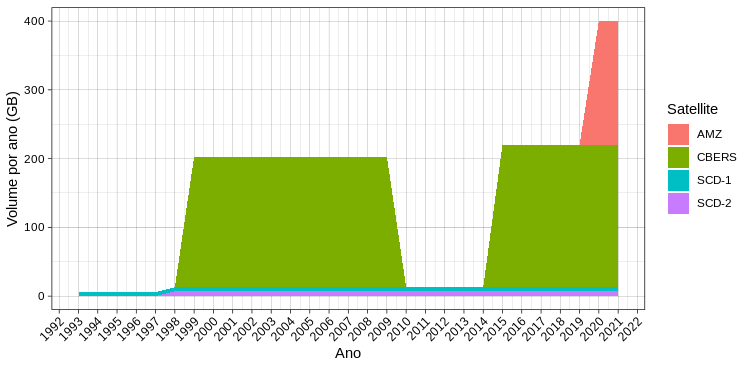
\includegraphics{Figuras/DataGenSatYear.png}}
	\end{center}
	\vspace{2mm}
	\legenda{Volume estimado de geração de dados por cada ano de operação de cada satélite.}
	\FONTE{Produção do autor.}
\end{figure}

Dessa estimativa, podemos obter o total de dados de telemetria disponíveis para a análise no CCS considerando uma taxa constante dos satélites, apresentados na figura~\ref{fig:totaldatagen}.
É importante ressaltar que a grande maioria desses dados não está disponível para consulta pelo usuário, visto que somente os dados de alguns poucos anos da operação estão disponíveis para os operadores e engenheiros, necessitando de trabalho significativo para analisar dados do passado.

\begin{figure}[!hb]
	\caption{Estimativa do volume de dados histórico de telemetria de todos os satélites}\label{fig:totaldatagen}
	\vspace{4mm}
	\begin{center}
		\resizebox{13cm}{!}{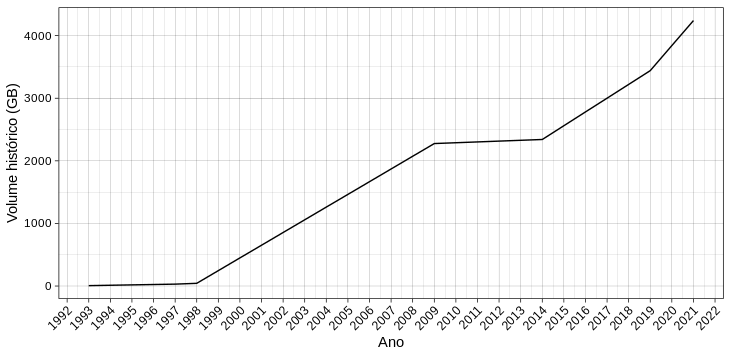
\includegraphics{Figuras/VolumeToYear.png}}
	\end{center}
	\vspace{2mm}
	\legenda{Volume total estimado de dados de telemetria gerados por todos os satélites.}
	\FONTE{Produção do autor.}
\end{figure}

Esses dados devem ser propriamente tratados para que não virem ``\textit{dark data}'', termo que denota quaisquer tipo de dados que não são de fácil acesso para os seus usuários em potencial~\cite{heidornSheddingLightDark2008}.

Esses dados entram na definição de \textit{Big Data}, pois possuem um grande volume, são gerados continuamente, possuem formatos diversos, sua análise é de alto valor e existe uma incerteza quanto a qualidade dos dados devido a problemas de comunicação e degradação dos instrumentos.
Essas características são denotadas pelos cinco Vs do \textit{Big Data}: Volume, Variedade, Velocidade, Valor e Veracidade~\cite{kacfahemaniUnderstandableBigData2015}.

Considerando que todos os dados já estivessem no banco de dados, propriamente formatados e prontos para a análise, ainda teríamos grandes problemas: com um banco de dados na ordem dos \textit{terabytes}, consultas multidimensionais ou que precisem de dados de vários anos poderiam demorar dias, ou mais, para serem executadas.

}

Deste modo, é necessário criar uma estrutura que permita a análise e consulta desses dados de uma forma estruturada e que tenha desempenho satisfatório.
As tecnologias de \textit{Data Warehouse} (DW) e \textit{Online Analytical Processing} (OLAP) tem demonstrado capacidade e experiência para atingir esses objetivos~\cite{bimonteOpenIssuesBig2016}, inclusive na área espacial~\cite{yvernesCopernicusGroundSegment2018}.
Essas tecnologias executam a generalização de dados agregando enormes quantidade de dados em vários níveis de abstração, assim tornam elementos essenciais de apoio à decisão e atraem a atenção tanto da indústria como das comunidades de pesquisa.
Sistemas OLAP, que são tipicamente dominados por consultas complexas que envolvem operadores \textit{group-by} e operadores de agregações, são as principais características entre essas ferramentas.

Sistemas OLAP são baseados em um modelo multidimensional chamado de cubo de dados, que é uma generalização do operador \textit{group-by} sobre todas as combinações possíveis das dimensões, com variados níveis de granularidade~\cite{grayDataCubeRelational1996}.
Cada combinação é chamada de um subcubo, que correspondem a um conjunto de células descritas como tuplas sobre as dimensões do subcubo.
Além das dimensões, cada tupla contém um fato, também chamado de medida, que representa o que será medido no processo de análise.

Cada dimensão pode estar organizada em uma hierarquia para facilitar a análise.
Por exemplo, uma dimensão tempo pode ser dividida em ``dia < mês < ano'', com ano sendo o nível mais genérico.
Essa prática visa facilitar a interpretação dos dados pelos usuários.
Medidas são atributos atributos associados a uma combinação de dimensões, sendo geradas de forma estatística.

Tecnologias OLAP são caracterizadas pela habilidade em responder consultas de apoio a decisão de forma eficiente.
Para atingir isso, o cubo de dados deve ser materializado antes da execução da consulta.
Isso significa que as combinações de dimensões são computadas previamente, assim gerando o cubo de dados completo.
Porém, essa abordagem possui um custo computacional exponencial em relação ao número de dimensões, assim a materialização completa do cubo envolve um grande número de células e um tempo substancial para a sua execução.

Dados de satélite são caracterizados pela sua alta dimensionalidade, onde um satélite pode precisar rastrear milhares de telemetrias.
Por exemplo, supondo um satélite com $n = 100$ telemetrias, e cada telemetria representando uma dimensão, teremos $2^{100}$ possíveis subcubos para a implementação de um cubo de dados.
Supondo uma cardinalidade, o número de valores diferentes em cada telemetria, como sendo de $100$, teremos $101^{100} \approx 10^{200}$ células para cada dimensão.
{\color{cerulean}
Devido ao controle ativo pelos operadores de satélite, os dados são concentrados em alguns valores que se repetem frequentemente, sendo que isso é chamado de \textit{skew}.
}

Dessa forma, conseguir calcular e manter um cubo de dados é um problema exponencial, e reduzir o seu consumo de memória e tempo de computação é de fundamental importância para desenvolver um sistema OLAP.
Para a área espacial essa necessidade é maior: a maior parte dos algoritmos de computação do cubo tem problemas em lidar com mais do que 15 dimensões~\cite{silva:2015:abordagensParaCubo}.

\section{Objetivos}\label{ch:intro:obj}

{\color{cerulean}

Assim, este trabalho tem como objetivo estabelecer um método para processamento de cubos de dados para a área espacial, para que o processamento de consultas OLAP sejam executadas de forma eficiente considerando-se a alta dimensionalidade, elevado número de tuplas, alto \textit{skew} e alta cardinalidade dos dados.

Assim é necessário identificar quais são as consultas de interesse dos operadores de satélite e quais são as análises que devem ser feitas pelos mesmos.
Disso será criada uma representação dimensional dos dados de telemetria em uma estrutura do cubo de dados, e  algoritmos de construção do cubo devem ser avaliados para identificar qual é o mais apropriado para responder as consultas.

Como resultados esperados deste trabalho teremos a avaliação dos algoritmos de construção do cubo nos dados altamente dimensionais, teremos as consultas identificadas e a adequabilidade do uso de cubo de dados como uma solução para operadores de satélites.

}

\section{Organização da proposta}\label{ch:intro:org}

Os capítulos restantes desta proposta estão organizados da seguinte maneira:

\begin{itemize}
	\item{Capítulo 2}: Este capítulo apresenta os conceitos e fundamentos teóricos desta proposta, como os conceitos relevantes de operação de satélites, \textit{Data Warehouse}, \textit{Big Data} e do Cubo de Dados.
	\item{Capítulo 3}: Neste capítulo os trabalhos correlatos de Cubo de Dados são apresentados, bem como as arquiteturas que outros operadores de satélite estão implementando.
	\item{Capítulo 4}: Neste capítulo a proposta é apresentada e seus conceitos principais explicados.
	\item{Capítulo 5}: Esse capítulo apresenta os resultados alcançados até o momento.
	\item{Capítulo 6}: Com base nos resultados intermediários alcançados, esse capítulo apresentará as conclusões obtidas, bem como as direções de implementação para o resto do trabalho.
\end{itemize}


%%%%%%%%%%%%%%%%%%%%%%%%%%%%%%%%%%%%%%%%%%%%%%%%%%%%%%%%%%%%%%%%%%%%%%%%%%%%%%

\chapter{THEORETICAL BACKGROUND}\label{ch:fun}

This chapter presents the theoretical background necessary to understand the concepts in this thesis, starting with satellite operations, the definitions of Big Data, Data Warehouse, OLAP and Data Cubes.

\section{Satellite Operations}\label{ch:fun:operations}

A satellite is divided into two modules: the service module and the payload.
The service module is composed of everything necessary for the operation of the on-board equipment, such as the power supply system, the ground communication system, the on-board computer, etc.
The payload is composed of all the necessary equipment to fulfill the mission objectives, these being sensors, cameras, telescopes, etc~\cite{larsonSpaceMissionAnalysis1999}.

A satellite generates two different types of data: payload data and telemetry data.
Payload data is the data generated to fulfill the mission of the satellite, and it can be photos taken for remote sensing, photos taken by telescopes, communication data if this is the focus of the mission among others~\cite{larsonSpaceMissionAnalysis1999}.
The telemetry data are the monitoring data of the health status and good operation of the satellite systems. These data are collected by the satellite's on-board computer, and are sent to the ground stations via telecommunication systems.

The telemetry data usually consist of sensor measurements on the satellite equipment, information collected by the on-board computer (such as whether an instrument is turned on or not), and other data whose collection has been defined as relevant to the operation of the satellite.
Depending on the mission, other measurements can be classified as telemetry, e.g. satellite-facing cameras, radars for the detection of possible collisions, etc~\cite{kragCmSpaceDebris2017}.

This data must be analyzed by satellite operators, who are responsible for monitoring and operating the satellite, on the ground after reception at the control center.
This analysis aims to ensure that the satellite is performing the tasks as it should, and that its state of health allows the continuation of the mission.

\section{Big Data}\label{ch:fun:bigdata}

The concept of Big Data is still evolving, and in this work the 5 Vs definition will be used: Volume, Variety, Velocity, Value and Veracity~\cite{kacfahemaniUnderstandableBigData2015}.

\begin{itemize}[noitemsep]
  \item \textbf{Volume}: This term generally specifies an amount of data in which a traditional database management system is ineffective.
  It is important to note that this is not only about the storage of data, but also about its processing~\cite{boussoufBigDataBased2018}.
  Using a large volume of data usually implies in better models, which are then hoped to produce better analyses, justifying the collection of a large amount of data.
  \item \textbf{Variety}: The data has multiple sources, with different formats, without a standardized modeling scheme, such as data coming from computertexts, sensor data, multimedia data, etc.
  As a consequence, these data should be used as transparently as possible in the analysis.
  \item \textbf{Velocity}: data is made available very quickly, and should be analyzed as quickly as possible.
  This implies that the data might be stored and analyzed even in real time.
  \item \textbf{Value}: data must be stored to create some value for its users, be it economic, scientific, social, organizational, etc.
  \item \textbf{Veracity}: the data has no guarantees as to its quality, such as inconsistencies and lack of accuracy, but the analysis must be of high quality anyway.
\end{itemize}

These V's are related to the construction of a Data Warehouse, and can also be seen as requirements for the creation of one for a data set characterized by Big Data~\cite{zhangBigDataFramework2017}.
In particular, there is a certain relationship with the idea of ``NoSQL'' (``Not only SQL''), where not only relational database systems are used, but also other paradigms are used, such as document oriented, key and value, etc~\cite{bimonteOpenIssuesBig2016}.

\section{Data Warehouse}\label{ch:fun:dw}

A Data Warehouse (DW) is a subject oriented, integrated, time-varying or time partitioned, non-volatile data repository that assists the decision making process~\cite{inmonUsingDataWarehouse1994}.
This definition can be divided into:

\begin{itemize}[noitemsep]
  \item \textbf{Subject oriented}: the DW is used for the analysis of a specific area.
    For example, a DW for telemetry data might just be useful for the operators, but not specific enough for engineering.
  \item \textbf{Integrated}: the DW must integrate data from multiple sources in a structured way.
    For example, even if there are two different representations for the same product, the DW should have only one representation.
    This requires the use of data cleaning and integration techniques in order to ensure data consistency.
  \item \textbf{Time-varying or time partitioned}: the DW must explicitly or implicitly contain the time perspective.
    This means that DW has historical data and they can be consulted during the analysis.
    For example, one might want to know data from days, months or years ago.
  \item \textbf{Non-volatile}: once inside DW, the data is not removed or updated, being a requirement for consulting historical data.
\end{itemize}

These features differentiate the Data Warehouse from other repository systems such as database systems, transaction processing systems and file systems~\cite{hanDataMiningConcepts2011}.

A DW is generally represented by a dimensional model that allows efficiency in data organization and management information retrieval~\cite{kimballDataWarehouseToolkit2013}.
Furthermore, this model has a few definitions: facts, dimensions and measures.
A fact corresponds to the business subject to be analyzed, each dimension is a visualization perspective of the business subject and measures are numerical values that quantify the business subject.
One of the dimensions is always temporal to allow the analysis of the subject over time.

\section{OLAP}\label{ch:fun:olap}

\textit{On-line Analytical Processing} (OLAP) is a term that refers to a set of tools that are used to summarize, consolidate, visualize, apply formulations and synthesize data according to multiple dimensions~\cite{coddProvidingOlapUseranalysts1998}.

An OLAP system allows the response of multi-dimensional queries using data stored in the Data Warehouse~\cite{kimballDataWarehouseToolkit2013}, and the main features are~\cite{bimonteOpenIssuesBig2016}:

\begin{itemize}[noitemsep]
  \item \textbf{Online queries}: must be made \textit{Online}, that is, in time for the user.
  \item \textbf{Multidimensional queries}: They are defined using the dimensions and measures provided by the Data Warehouse, which expect high quality data.
  \item \textbf{Simple representation}: Query results must be represented using tables and graphs, because end users are usually decision makers who need visualizations that are relevant to the subject.
  \item \textbf{Exploratory}: queries are used in an exploratory way, since users generally do not know in advance all the data available for queries.
\end{itemize}

Each OLAP tool must manipulate a new Abstract Data Type (ADT), called a data cube, using specific strategies due to the way the data is stored, being classified in~\cite{moreiraFullPartialData2012}:

\begin{itemize}[noitemsep]
  \item \textbf{Relational OLAP (ROLAP)}: use relational Database Management Systems (Data base Management System - DBMS) for the management and storage of data cubes.
    ROLAP tools include optimizations for each DBMS, implementation of navigation logic in aggregations, services and additional tools;
  \item \textbf{Multidimensional OLAP (MOLAP)}: implement multidimensional data structures to store data cubes in main memory or in external memory.
    No relational repositories are used to store multidimensional data and the navigation logic is already integrated into the proposed structure;
  \item \textbf{Hybrid OLAP (HOLAP)}: combine ROLAP and MOLAP techniques, where detailed data is stored in a relational database (ROLAP), and aggregations are stored in multidimensional data structures (MOLAP).
\end{itemize}

It is important to highlight the difference between OLAP and Online Transaction Processing (OLPT), since common database systems use only OLTP, which has the purpose of performing valid transactions and processing queries.
This covers the vast majority of day-to-day operations, such as stock control, banking operations, etc., serving various users of an organization.
OLAP is used by decision makers and data analysts and is geared towards higher level decisions in the organization~\cite{hanDataMiningConcepts2011}.

\section{Data Cube}\label{ch:fun:cube}

The data cube was originally created as a relational operator that generates all the possible combinations of its attributes according to a measure~\cite{grayDataCubeRelational1996}.

The structure of the data cube allows the data to be modeled and visualized in multiple dimensions, and it is characterized by dimensions and measures.
A measurement is an attribute whose values are calculated by the relationship between the dimensions, which is calculated using aggregation functions such as sum, count, average, mode, median, etc.
A dimension is made by the entities that compose the data, determining the context of the subject in question.
A dimension can also be divided into members, which can have a hierarchy, such as a time dimension divided in day, month and year~\cite{hanDataMiningConcepts2011}.

The organization of a data cube allows the user the flexibility to visualize the data from different perspectives, since the cube operator generates combinations through the concept of the value \textit{ALL}, where this concept represents the aggregation of all possible combinations of a set of attribute values.
Operations in data cubes exist in order to materialize these different views, allowing search and interactive analysis of stored data~\cite{hanDataMiningConcepts2011}.

A data cube is composed of cells and each cell has values for each dimension, including \textit{ALL}, and values for the measurements.
\autoref{fig:cubeexample} shows an example of a data cube.
The value of a measure is computed for a given cell using lower aggregation levels to generate the values of the higher aggregation levels in the \textit{Top-down} strategy, with the inverse order used in \textit{Bottom-up}.

\begin{figure}[!htb]
  \caption{Data Cube example}\label{fig:cubeexample}
  \vspace{2mm}
  \begin{center}
    \resizebox{9cm}{!}{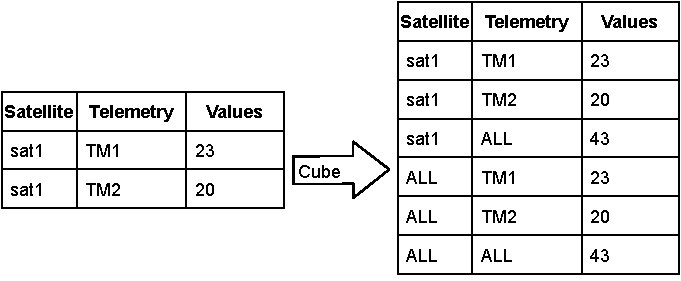
\includegraphics{Figuras/CubeExample.pdf}}
  \end{center}
  \vspace{1mm}
  \legenda{}
  \FONTE{Author}
\end{figure}

\subsection{Data Cube Cells}\label{ch:fun:cube:cells}

A data cube is composed of several subcubes, which are all possible levels of aggregation in the specified dimensions.
Subcubes are composed of base cells and aggregated cells, and an aggregated cell is a cell that uses the special value \textit{ALL} (``$*$'') to demonstrate that it is adding values in one or more dimensions.
A base cell does not use the \textit{ALL} notation, being composed of the lowest level of aggregation~\cite{limaSEQUENTIALPARALLELAPPROACHES2009}.
\autoref{fig:hasse} shows all levels of aggregation of a cube composed of dimensions A, B and C, from the most generic (\textit{apex}) to the most specific (base).

\begin{figure}[!htb]
  \caption{All subcubes for a three dimensional cube}\label{fig:hasse}
  \vspace{2mm}
  \begin{center}
    \resizebox{5cm}{!}{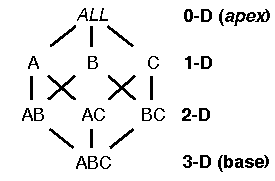
\includegraphics{Figuras/Hasse.pdf}}
  \end{center}
  \vspace{1mm}
  \legenda{A Hasse Diagram of a data cube with three dimensions A, B and C.}
  \FONTE{Author}
\end{figure}

Formally, assuming a $n$-dimensional data cube, a cell $a$ of any subcube is defined by $a = (a_1, a_2, a_3, \ldots, a_n, measures)$.
The cell is $m$-dimensional (from a subcube with $m$ dimensions), if exactly $m$, with $(m \leq n)$, values between $(a_1, a_2, a_3, \ldots, a_n)$ are not ``$*$''.
If $m = n$, then $a$ is a base cell, otherwise $(m < n)$, it is an aggregate cell.

A descending-ancestral relationship can exist between cells.
In a $n$-dimensional data cube, a cell $a = (a_1, a_2, a_3, \ldots, a_n, measures_a)$ with level $i$ is an ancestor of a cell $b = (b_1, b_2, b_3, \ldots, b_n, measures_b)$ of level $j$, and $b$ is a descendant of $a$, if and only if $i < j$ and $1 \leq m \leq n$, where $a_m = b_m$ whenever $a_m \neq *$.
In particular, a $a$ cell is called the parent of a $b$ cell, and $b$ the child of $a$, if and only if $j = i+1$ and $b$ is a descendant of $a$~\cite{hanDataMiningConcepts2011}.

\subsection{Dimensional Modelling}\label{ch:fun:cube:dimm}

There are three main schemes for the dimensional modeling of a data cube: Star Schema, Snowflake Schema and Fact Constellation.
The star schema is the most used, as it contains a central table called the fact table, where most of the data is located, with a smaller set of tables, called dimension tables, for the other dimensions.
\autoref{fig:starschema} shows an example of a star scheme.

\begin{figure}[!htb]
  \caption{Star schema}\label{fig:starschema}
  \vspace{6mm}
  \begin{center}
    \resizebox{4cm}{!}{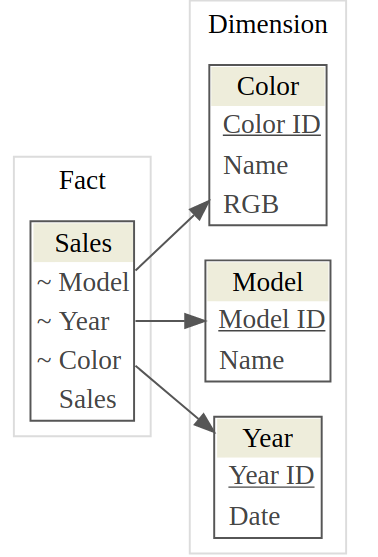
\includegraphics{Figuras/starSchema.png}}
  \end{center}
  \vspace{1mm}
  \legenda{}
  \FONTE{Author}
\end{figure}

The snowflake scheme is a variation of the star scheme, where some dimensions are normalized, dividing the data of the dimension tables into other tables.
This has the advantages of eliminating redundancies in the dimension tables, but it creates problems during the execution of queries since it is necessary to perform join operations with the new tables.
\autoref{fig:snowflakeschema} shows an example of a snowflake scheme.

\begin{figure}[!htb]
  \caption{Snowflake schema}\label{fig:snowflakeschema}
  \vspace{2mm}
  \begin{center}
    \resizebox{6cm}{!}{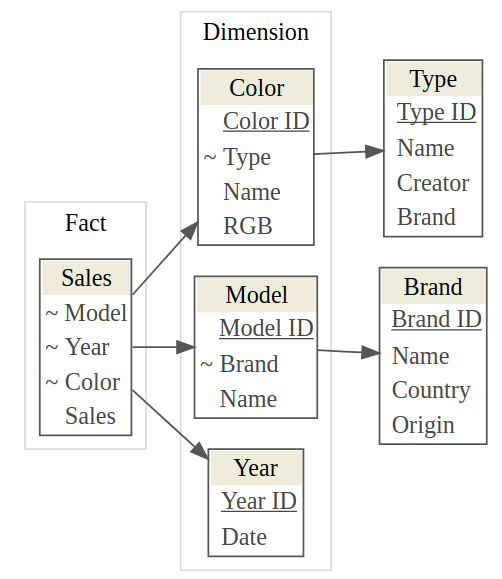
\includegraphics{Figuras/snowflakeSchema.png}}
  \end{center}
  \vspace{1mm}
  \legenda{}
  \FONTE{Author}
\end{figure}

The Fact Constellation uses multiple fact tables, like multiple star schemas but sharing dimension tables, leading to its name as a group of stars.
\autoref{fig:factconstschema} shows an example of a fact constellation scheme.

\begin{figure}[!htb]
  \caption{Fact Constellation scheme}\label{fig:factconstschema}
  \vspace{6mm}
  \begin{center}
    \resizebox{6cm}{!}{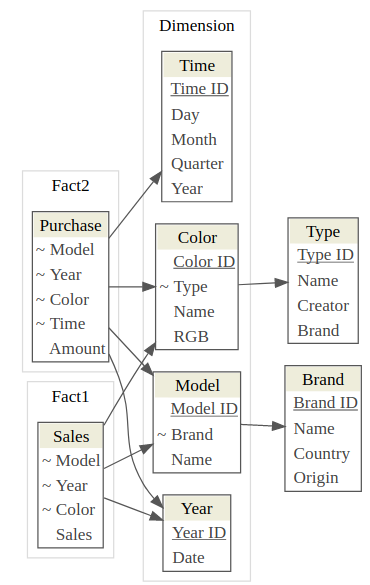
\includegraphics{Figuras/factConstellationSchema.png}}
  \end{center}
  \vspace{2mm}
  \legenda{}
  \FONTE{Author}
\end{figure}

\subsection{Concept Hierarchies}\label{ch:fun:cube:concept}

A concept hierarchy is used to define a mapping sequence between a set of low-level concepts and a set of high-level, more general concepts.
It is a style of grouping and discretization, because it groups the values in order to reduce the cardinality of a dimension~\cite{hanDataMiningConcepts2011}.
They help make the analysis easier to understand, as the operations translate the low-level data into a representation that is easier for the end user, thus facilitating the execution of queries and their subsequent use.

\subsection{Measures}\label{ch:fun:cube:measures}

Each cell of a cube is defined as a pair $\langle (d_1, d_2, \ldots, d_n), measures \rangle$, where $(d_1, d_2, \ldots, d_n)$ represent the possible combinations of attribute values over dimensions.
A measure is calculated for a certain cell by aggregating the data corresponding to the combination of dimensions and values~\cite{hanDataMiningConcepts2011}.
Measurements can be classified into three types: distributive, algebraic and holistic.

A distributive measure is a measure whose calculation can be partitioned and then combined, and the result would be the same if the calculation was performed on the entire data set.
For example, the sum function is distributive: dividing the $N$ data into $n$ sets, and making the sum of each $n$ set, will have the same result as if it were done directly over $N$.

An algebraic measure is a measure that can be calculated with two or more distributive measures.
For example, a measure of average can be calculated by dividing the measure sum by the measure count, which are both distributive.

A measure is holistic if there is no algebraic measure with $M$ arguments that performs the computation.
This means that computing cannot be partitioned, with exact values obtained only if the measure is applied to all data.
Some examples are the measures of mode, standard deviation and median~\cite{hanDataMiningConcepts2011}.

\subsection{OLAP Operations}\label{ch:fun:cube:olapops}

To perform queries in the Data Warehouse, it is necessary to use some operations on the data cube to obtain the appropriate results.
These queries must also be able to go through the hierarchy of concepts of each dimension, as well as follow the dimensional model of the cube, in order to offer a user-friendly interface for interactive analysis~\cite{hanDataMiningConcepts2011}.
Some operations are exemplified in \autoref{fig:olap}, but they usually are:

\begin{itemize}[noitemsep]
  \item \textit{Roll-up}: performs aggregation in the data cube, either by navigating the concept hierarchy from a specific level concepts to a more generic one, or by reducing a dimension.
  \item \textit{Drill-down}: the inverse of the roll-up operation, navigates in the hierarchy of concepts from the most generic level to the most specific level, or adds dimensions to the current cube.
  \item \textit{Slice}: performs a selection in a cube dimension, resulting in a subcube focused on that dimension.
  \item \textit{Dice}: defines a subcube by making a selection (slice) in two or more dimensions.
  \item \textit{Pivot}: also called rotation, it allows changing the position of the dimensions in view, changing rows to columns and vice versa.
\end{itemize}

\begin{figure}[!htb]
  \caption{OLAP operations in a Data Cube}\label{fig:olap}
  \vspace{4mm}
  \begin{center}
    \resizebox{15cm}{!}{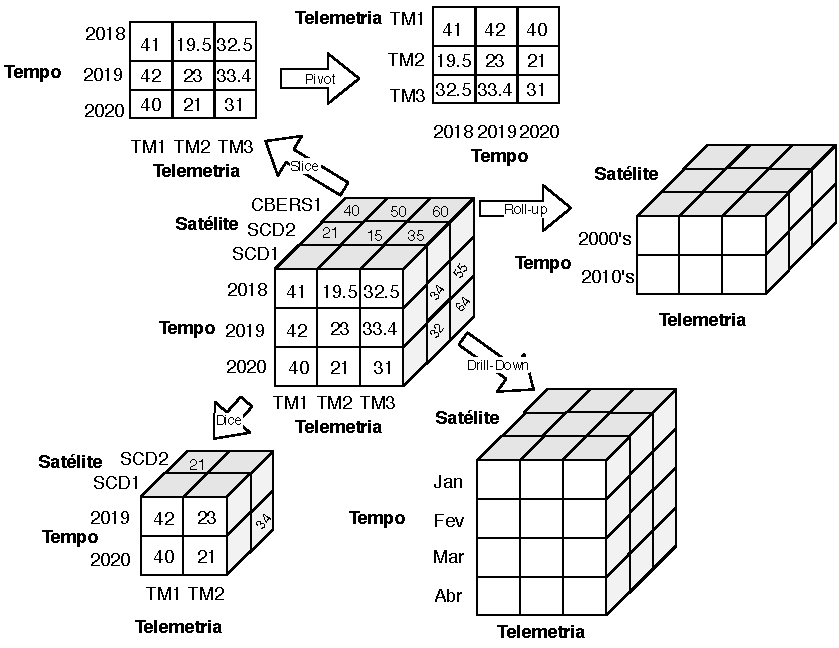
\includegraphics{Figuras/OLAP.pdf}}
  \end{center}
  \vspace{2mm}
  \legenda{Common OLAP operations on a three-dimensional data cube with Satellite, Time and Telemetry dimensions}
  \FONTE{Author}
\end{figure}

Depending on the OLAP system, it is possible to execute other operations, like drill-across between multiple fact tables, and drill-through where queries are executed directly on the low-level representation of the data~\cite{hanDataMiningConcepts2011}.

\subsection{Data Cube Computation}\label{ch:fun:cube:comp}

Data cube computation is an essential task, as pre-computing all or part of a data cube can significantly increase DW performance.
However, this task has exponential complexity in relation to the number of dimensions, being called materialization, with complete materialization requiring a large number of cells, and therefore a high consumption of memory and time~\cite{hanDataMiningConcepts2011}.

The original calculation of the data cube computation was proposed by~\citeonline{grayDataCubeRelational1996}, being: given an input relation $R$ with tuples of size $n$, the number of subcubes that can be generated is $2^n$, where $n$ is the number of dimensions of the cube.
For example, assuming a cube with three dimensions \textit{Satellite, Telemetry, Value}, we have $2^3 = 8$ possible subcubes: $\{(satellite, telemetry, value), (satellite, value), (satellite, telemetry),$ $(telemetry, value), (telemetry), (value), (satellite), \emptyset \}$, with $\emptyset$ denoting the empty grouping (base cell, dimensions are not grouped).
% Weird latex thing here...

However, in practice, dimensions can have associated concept hierarchies, as for the time dimension: ``day<month<quarter<semester<year'.
For a cube with $n$ dimensions with multiple concept hierarchies, the total number of subcubes is shown in \autoref{eq:conceptcuboids}.

\begin{equation}
  subcubes = \prod_{i=1}^n (L_i + 1)
\label{eq:conceptcuboids}
\end{equation}

Where $L_i$ is the number of concept levels of the $i$ dimension.
It is necessary to add one to the equation~\ref{eq:conceptcuboids} to denote the virtual level \textit{ALL}.
The size of each subcube also depends on the cardinality of each dimension, that is, the number of distinct values.
While the number of dimensions, concept hierarchies, and cardinality of the cube increases, they also increase the space requirements exponentially, being known as the \textbf{Curse of Dimensionality} in computing.

To be able to answer the queries properly, it is necessary to choose a method for subcube computing: non-materialisation, complete materialisation and partial materialisation.

In non-materialisation, the aggregated subcubes are not pre-computed, so the aggregations are computed in query time, which can be extremely slow, but has the lowest memory consumption.

Complete materialization computes all possible aggregations of the cube, generating a complete data cube.
This method generates the best response times, because the aggregations have already been computed, but it requires a large amount of memory.

Partial materialization only computes a selected subset of subcubes, and there are several different techniques for selecting the subcubes to be computed.
One of them is to compute all the subcubes that contain only cells that satisfy a given criterion, specified by the user.
These cubes are called iceberg~\cite{beyerBottomupComputationSparse1999}.

Another technique is to compute small cubes, usually between 3 and 5 dimensions, to form complete cubes.
To answer queries with more dimensions, the combinations between the small subcubes are aggregated.
This technique is called shell fragment, and the cube is called cube shell~\cite{liHighdimensionalOLAPMinimal2004}.

A data cube where cells with identical measurements are encapsulated in a single abstraction, called a closed cell is called a closed cube~\cite{dongxinCCubingEfficientComputation2006}, or quotient cube~\cite{lakshmananQuotientCubeHow2002}.

The choice of partial materialization depends on the required balance between response time and storage space.
However, full cube computation remains relevant, and advances in partial cube computation are generally adopted in full cube computation.
There is also the problem of updating the cube, as each update can cause a partial or complete recomputation of the cube to maintain the correct measurements.

From a base cube, the data cube computation can use the Top-down or Bottom-up strategy for the generation of the remaining subcubes~\cite{hanDataMiningConcepts2011}.

\autoref{fig:topdown} shows the generation of a four-dimensional data cube by the Top-down strategy.
ABCD being a base cube, the three dimension subcubes are: ABC, ABD, ACD and BCD; which can use the results of the base cube to be computed.

\begin{figure}[!hbt]
  \caption{Computing the data cube with the Top-Down strategy}\label{fig:topdown}
  \vspace{4mm}
  \begin{center}
    \resizebox{7cm}{!}{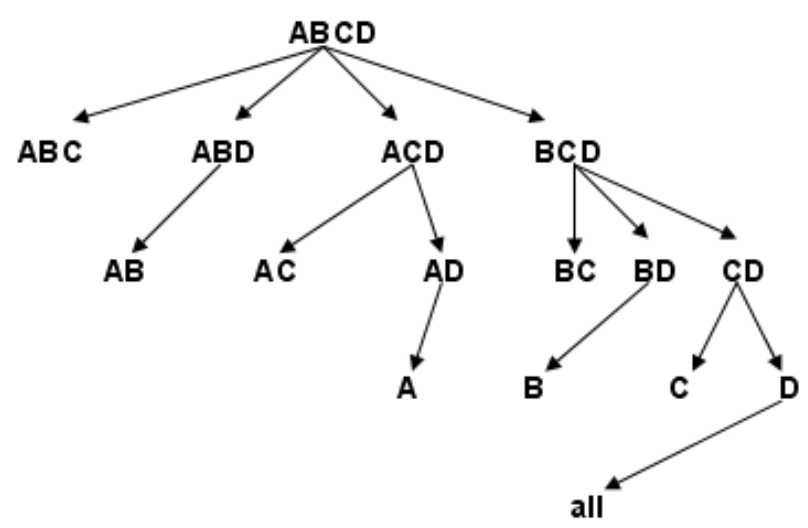
\includegraphics{Figuras/topdown.png}}
  \end{center}
  \vspace{2mm}
  \legenda{}
  \FONTE{~\cite{silva:2015:abordagensParaCubo}.}
\end{figure}

Os resultados da computação do subcubo ACD podem ser utilizados para computar AD, que consequentemente podem ser utilizados para computar A.
Essa computação compartilhada permite que a estratégia \textit{Top-down} compute agregações em múltiplas dimensões.
Os valores agregados intermediários podem ser reutilizados para a computação de subcubos descendentes sucessivos.

A Figura~\ref{fig:bottomup} mostra a geração de um cubo de dados de 4 dimensões por meio da estratégia \textit{Bottom-up}.
Subcubos de poucas dimensões tornam-se pais de subcubos com mais dimensões.
Infelizmente, a computação compartilhada, utilizada na estratégia \textit{Top-down}, não pode ser aplicada quando utilizada a estratégia \textit{Bottom-up}, então cada subcubo descendente necessita ser computado do início.

The results of the ACD subcube computation can be used to compute AD, which consequently can be used to compute A.
This shared computing allows the Top-down strategy to compute aggregations in multiple dimensions.
The intermediate aggregated values can be reused for the computation of successive descending subcubes.

\autoref{fig:bottomup} shows the generation of a 4-dimensional data cube through the Bottom-up strategy.
Low dimensional subcubes become parents of more dimensioned subcubes.
Unfortunately, the shared computing used in the Top-down strategy cannot be applied when using the Bottom-up strategy, so each descending subcube needs to be computed from the beginning.

\begin{figure}[!htb]
  \caption{Computing the data cube with the Bottom-Up strategy}\label{fig:bottomup}
  \vspace{4mm}
  \begin{center}
    \resizebox{8cm}{!}{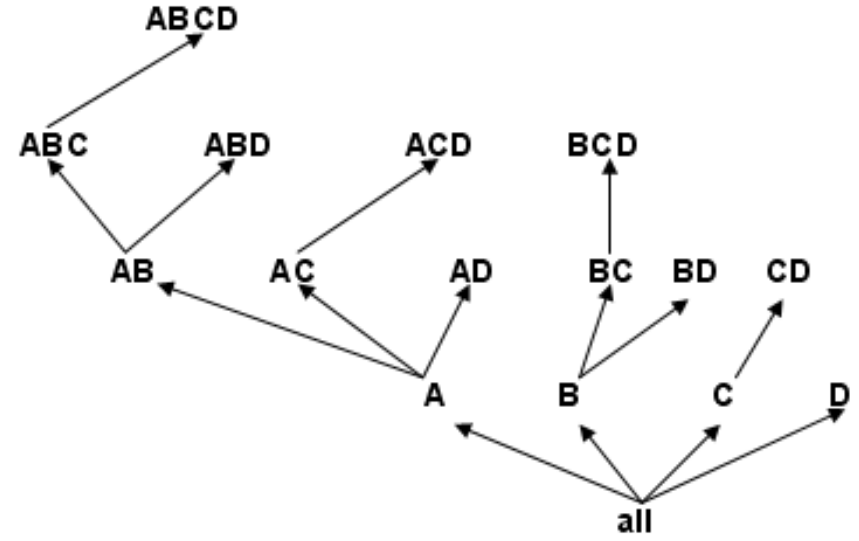
\includegraphics{Figuras/bottomup.png}}
  \end{center}
  \vspace{2mm}
  \legenda{}
  \FONTE{~\cite{silva:2015:abordagensParaCubo}.}
\end{figure}


%%%%%%%%%%%%%%%%%%%%%%%%%%%%%%%%%%%%%%%%%%%%%%%%%%%%%%%%%%%%%%%%%%%%%%%%%%%%%%%

\chapter{PROPOSTA}

Os capítulos restantes desta dissertação estão organizados da seguinte maneira:
\begin{itemize}
\item{Capítulo 2}: A Seção~\ref{seccaos} aborda, por meio de sistemas-paradigma de comportamento caótico como o Mapa Logístico e as Equações de Lorenz, as principais características apresentadas por sistemas dinâmicos não-lineares caóticos. A Seção~\ref{secturb} é destinada, em grande parte, à descrição fenomenológica da turbulência. São ainda apresentadas alguns temas de grande relevância no estudo da turbulência, como o fenômeno da intermitência e as estruturas coerentes. Finalmente, a Seção~\ref{seccaosurb} expõe uma perspectiva adicional para a compreensão do fenômeno turbulento com base na teoria de sistemas dinâmicos, mais especificamente por meio de atratores caóticos~\cite{ruelltak/71}.
\item{Capítulo 3}: Neste capítulo é feita uma descrição detalhada dos métodos e dos algoritmos disponíveis para a caracterização de caos determinístico presente em séries temporais experimentais. O tema é bastante extenso e especializado; como conseqüência, tal descrição será focada nos procedimentos mais utilizados para a reconstrução da dinâmica, para o cálculo de dimensão de atratores e do espectro de expoentes de Lyapunov. São abordados alguns problemas e limitações, do ponto de vista numérico, associados aos algoritmos utilizados, como também as dificuldades encontradas no tratamento de sinais experimentais. 
\item{Capítulo 4}: Neste capítulo é realizada uma breve descrição dos dados coletados pela campanha WETAMC do projeto LBA, bem como do sítio experimental.
\item{Capítulo 5}: Neste capítulo são aplicadas diversas ferramentas (descritas no Capítulo~\ref{caputiltecnicas}) nas séries temporais em estudo, em busca de atratores caóticos de baixa dimensão na camada limite atmosférica.
\item{Capítulo 6}: Com base nas análises realizadas no Capítulo~\ref{capanaliseseresults}, neste capítulo serão apresentadas as conclusões obtidas, como também algumas sugestões para trabalhos futuros.
\end{itemize}


%%%%%%%%%%%%%%%%%%%%%%%%%%%%%%%%%%%%%%%%%%%%%%%%%%%%%%%%%%%%%%%%%%%%%%%%%%%%%%%

\chapter{IMPLEMENTAÇÃO}

Os capítulos restantes desta dissertação estão organizados da seguinte maneira:
\begin{itemize}
\item{Capítulo 2}: A Seção~\ref{seccaos} aborda, por meio de sistemas-paradigma de comportamento caótico como o Mapa Logístico e as Equações de Lorenz, as principais características apresentadas por sistemas dinâmicos não-lineares caóticos. A Seção~\ref{secturb} é destinada, em grande parte, à descrição fenomenológica da turbulência. São ainda apresentadas alguns temas de grande relevância no estudo da turbulência, como o fenômeno da intermitência e as estruturas coerentes. Finalmente, a Seção~\ref{seccaosurb} expõe uma perspectiva adicional para a compreensão do fenômeno turbulento com base na teoria de sistemas dinâmicos, mais especificamente por meio de atratores caóticos~\cite{ruelltak/71}.
\item{Capítulo 3}: Neste capítulo é feita uma descrição detalhada dos métodos e dos algoritmos disponíveis para a caracterização de caos determinístico presente em séries temporais experimentais. O tema é bastante extenso e especializado; como conseqüência, tal descrição será focada nos procedimentos mais utilizados para a reconstrução da dinâmica, para o cálculo de dimensão de atratores e do espectro de expoentes de Lyapunov. São abordados alguns problemas e limitações, do ponto de vista numérico, associados aos algoritmos utilizados, como também as dificuldades encontradas no tratamento de sinais experimentais. 
\item{Capítulo 4}: Neste capítulo é realizada uma breve descrição dos dados coletados pela campanha WETAMC do projeto LBA, bem como do sítio experimental.
\item{Capítulo 5}: Neste capítulo são aplicadas diversas ferramentas (descritas no Capítulo~\ref{caputiltecnicas}) nas séries temporais em estudo, em busca de atratores caóticos de baixa dimensão na camada limite atmosférica.
\item{Capítulo 6}: Com base nas análises realizadas no Capítulo~\ref{capanaliseseresults}, neste capítulo serão apresentadas as conclusões obtidas, como também algumas sugestões para trabalhos futuros.
\end{itemize}


%%%%%%%%%%%%%%%%%%%%%%%%%%%%%%%%%%%%%%%%%%%%%%%%%%%%%%%%%%%%%%%%%%%%%%%%%%%%%%%

\chapter{CONCLUSÃO}

Este trabalho apresenta uma arquitetura baseada em conceitos de \textit{Big Data} para auxiliar nas atividades de análise para operadores de satélites. Conceitos e definições importantes da área são especificados, bem como uma revisão é feita na literatura de como outros operadores de satélite estão utilizando essas tecnologias.

Também são apresentados resultados intermediários de análises e softwares feitos para prototipar as operações de análise [...?]

\textbf{Como essa arquitetura é melhor(diferente?) da utilizada por outros operadores? O que o Cubo de Dados traz de diferente?}

\textbf{Planos futuros, o que vai ser implementado daqui para frente}



%% insira quantos capítulos desejar com o seguinte comando:
%\include{_pasta_do_arquivo_/_meu_arquivo_} %%sem a extensão
%% note que deverá haver um arquivo _meu_arquivo_.tex (com extensão) no diretório _pasta_do_arquivo_

%\include{./docs/conclusao}

%% Bibliografia %% não alterar %% obrigatório %testebib
\bibliography{./bib/EXAM} %% aponte para seu arquivo de bibliografia no formato bibtex (p.ex: referencia.bib)


%\include{./docs/glossario} %% insira os termos do glossário no arquivo glossario.tex %% opcional

%\inicioApendice %% opcional, comente esta linha e a seguintes se não houver apendice(s)
%%%%%%%%%%%%%%%%%%%%%%%%%%%%%%%%%%%%%%%%%%%%%%%%%%%%%%%
%Apêndice A
\hypertarget{estilo:apendice1}{} %% uso para este Guia
%Este apêndice foi criado apenas para indicar como construir um apêndice no estilo, não existia no original da tese.
%%%%%%%%%%%%%%%%%%%%%%%%%%%%%%%%%%%%%%%%%%%%%%%%%%%%%%
\renewcommand{\thechapter}{}%
\chapter{APÊNDICE A - AUTORIZAÇÃO PARA PUBLICAÇÃO}	% trocar A por B na próxima apêndice e etc
\label{apendiceA}	% trocar A por B na próxima apêndice e etc
\renewcommand{\thechapter}{A}%		% trocar A por B na próxima apêndice e etc

Há dois formulários de autorização para publicação, um para publicações de trabalhos acadêmicos e outro para publicações técnico-científicas, neste apêndice encontram-se os modelos dos formulários e suas respectivas instruções de preenchimento. 

\section{Autorização para Publicação de Trabalho Acadêmico - INPE-393}

\label{instr393}

	\begin{figure}[ht]
		\caption{Formulário Autorização para Publicação de Trabalho Acadêmico INPE-393.}
		\vspace{6mm}	% acrescentar o espaçamento vertical apropriado entre o título e a borda superior da figura
		\centering
   		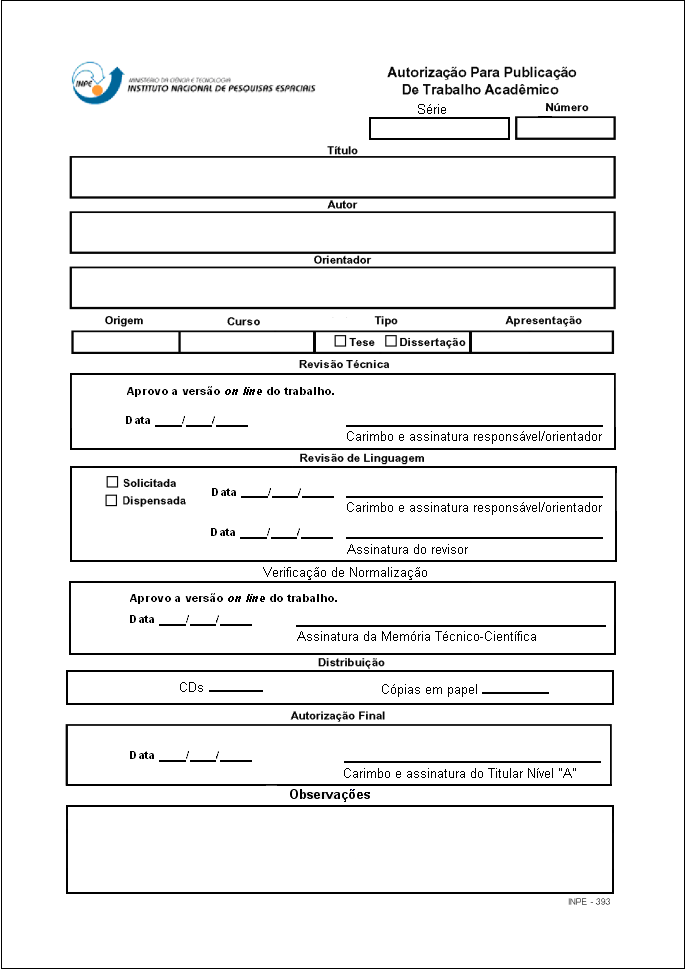
\includegraphics[height=16cm]{./Figuras/form393.png}	   
 		\label{form393}
	\end{figure}


\subsection{Instruções do Formulário INPE-393} 

\begin{enumerate} 

 \item \textbf{série:} com este número o SID identifica as publicações do INPE, composto da sigla da Instituição, número sequencial geral da publicação, sigla e número sequencial do tipo de publicação, exemplo: INPE-14209-TDI/1110;
 
 \item \textbf{número:} será composto da sigla da unidade do SID, mais 4 (quatro) dígitos e do ano em curso. Este número de referência é de controle da unidade emissora. Ex.: SID-0001/2007;

 \item \textbf{título da publicação:} deve ser completo, evitando-se abreviar palavras;

 \item \textbf{nome do autor e do orientador:} estes campos devem ser preenchidos por extenso, da mesma forma em que irão constar da publicação;

 \item \textbf{origem da publicação:} sigla da unidade do servidor (autor da publicação), conforme TQ-001;

 \item \textbf{curso:} sigla do curso, de acordo com a Estrutura de Divisão de Trabalho - EDT do INPE;
 
 \item \textbf{tipo:} assinalar se é tese ou dissertação;

 \item \textbf{apresentação:} colocar a data de aprovação final;

 \item \textbf{revisão técnica:} o responsável designado pela Banca Examinadora para verificação de correções e, na ausência desse, o orientador da tese ou dissertação deve
carimbar, datar e assinar após a versão \emph{on line} do trabalho;

 \item \textbf{revisão de linguagem:} o responsável designado pela Banca Examinadora para verificação de correções, e na ausência deste o orientador deve assinalar a solicitação ou a dispensa da revisão de linguagem e, carimbar, datar e assinar; o revisor deve datar e assinar após a revisão;
 
 \item \textbf{distribuição:} O SID deve informar a quantidade de CD's e de cópias impressas da tese ou dissertação, conforme lista de distribuição;
 
 \item \textbf{verificação de normalização:}  Após a verificação da versão \emph{on line} do trabalho quanto às normas editoriais, o SID deve datar e assinar;
 
 \item \textbf{autorização final:} data e assinatura do Titular de Nível A, conforme TQ-001, a que o Serviço de Pós-Graduação estiver subordinado.
 
 \item \textbf{observações:} para outras informações necessárias. 

\end{enumerate}

\section{Autorização para Publicação - INPE-106}
\begin{figure}[ht!]
	\caption{Formulário Autorização para Publicação de Trabalho Acadêmico INPE-106 folha 1.} 
	\vspace{6mm}	% acrescentar o espaçamento vertical apropriado entre o título e a borda superior da figura
	\centering
	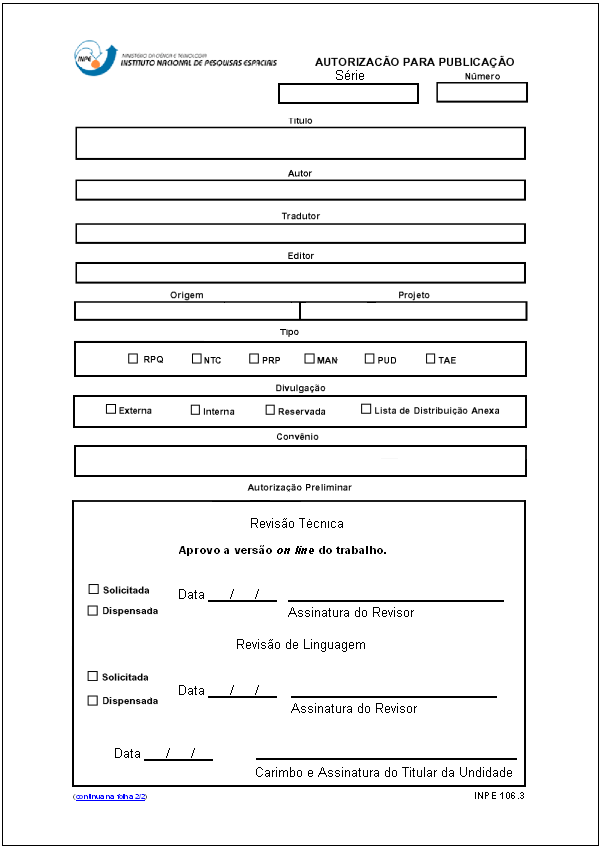
\includegraphics[height=18cm]{./Figuras/form106.png}
	\label{form106}
\end{figure}

\begin{figure}[ht!]
	\caption{Formulário Autorização para Publicação de Trabalho Acadêmico INPE-106 folha 2.} 
	\vspace{6mm}	% acrescentar o espaçamento vertical apropriado entre o título e a borda superior da figura
	\centering
	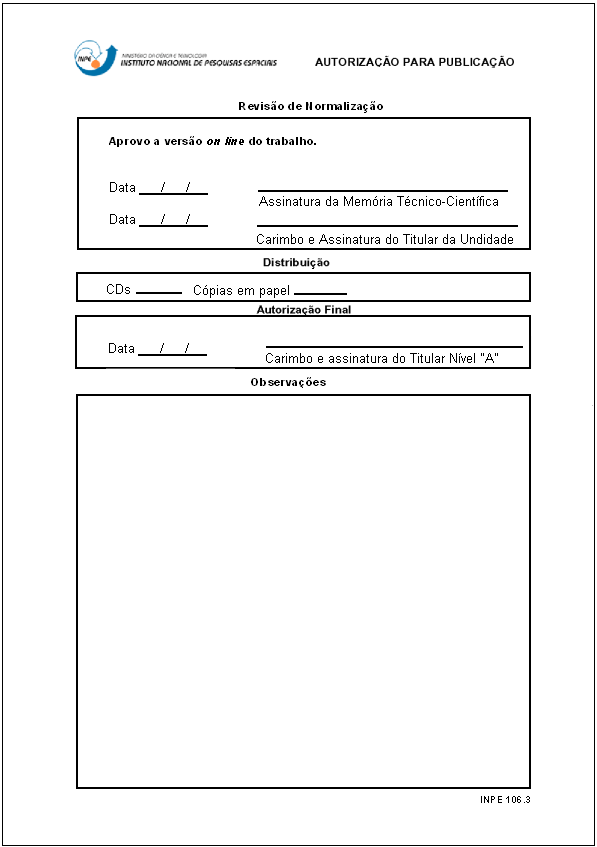
\includegraphics[height=18cm]{./Figuras/form106folha2.png}
	\label{form106a}
\end{figure}

\clearpage
\subsection{Instruções do Formulário INPE-106} 
\label{instr106}


\begin{enumerate}

 \item \textbf{série:} com este número o SID identifica as publicações do INPE, composto da sigla da Instituição, número sequencial geral da publicação, sigla e número sequencial do tipo de publicação, exemplo: INPE-5616-RPQ/671. 
 
 \item \textbf{número:} será composto da sigla da unidade constante da Estrutura Organizacional do INPE (TQ-001), mais 4 (quatro) dígitos e do ano em curso. Este número de referência é de controle da unidade solicitante. Ex: CEA-0001/2007;
 
 \item \textbf{título da publicação:} deve ser completo, evitando-se abreviar palavras;

 \item \textbf{nome do autor, tradutor e editor:}  estes campos devem ser preenchidos por extenso, da mesma forma em que irão constar da publicação;

 \item \textbf{origem da publicação:} sigla da unidade do servidor (autor da publicação), conforme TQ-001;

 \item \textbf{projeto:} sigla do projeto de acordo com a Estrutura de Divisão de Trabalho - EDT do INPE;

 \item \textbf{tipo de publicação:} assinalar o tipo de publicação proposta:

 \begin{enumerate}
  \item{Relátorio de Pesquisa (RPQ)},
  \item{Notas Técnico-Científicas (NTC)},
  \item{Propostas e Relatórios de de Projeto (PRP)},
  \item{Manuais Técnicos (MAN)},
  \item{Publicações Didáticas (PUD)},
  \item{Trabalhos Acadêmicos Externos (TAE)}.
 \end{enumerate}

 \item \textbf{divulgação:} assinalar, de acordo com os critérios de classificação. Se houver Lista de Divulgação, nesta deverá constar os nomes e endereços completos;

 \item \textbf{convênio:} descrever o nome da instituição, quando a publicação for realizada pelo INPE e outra organização, preencher somente para o tipo PRP; 
 
    \item \textbf{autorização preliminar:} data, carimbo e assinatura do Titular da Unidade a que o autor esteja subordinado e, assinatura do revisor que efetuou a revisão técnica aprovando a versão \emph{on line} do trabalho e do revisor que realizou a revisão de linguagem, quando solicitadas; 
    
  \item \textbf{verificação de normalização:} o SID deve datar e assinar após a revisão da adequação às normas editoriais;   
  
  \item \textbf{distribuição:} O SID deve informar a quantidade de CD's e de cópias impressas que deverão ser gravados conforme lista de distribuição;
  
 \item \textbf{autorização final:} data, carimbo e assinatura do Titular de Nível "A", conforme TQ-001, a que o autor da publicação estiver subordinado;
 
 \item \textbf{observações:} para outras informações necessárias, inclusive para descrever as justificativas de uma publicação.
\end{enumerate} %% insira apendices tal qual capítulos acima

\inicioAnexo
%%%%%%%%%%%%%%%%%%%%%%%%%%%%%%%%%%%%%%%%%%%%%%%%%%%%%%%%%%%%%%%%%%%%%%%%%%%%%%%%%

\renewcommand{\thechapter}{}%
\chapter{ANEXO A - CRONOGRAMA}
\label{anexoA}
\renewcommand{\thechapter}{A}

\begin{table}[!ht]
  \label{tab:cronograma}
  \begin{center}
	\caption{Cronograma de atividades}
	\begin{tabular*}{\textwidth}{|p{3cm}|c|c|c|c|c|c|c|c|c|c|} %%11!
		\hline
		\textbf{Atividade} & maio & jun. & jul. & ago. & set. & out. & nov. & dec. & jan. & fev. \\
		\hline
		Entrevista de qualificação &X&&&&&&&&& \\
		\hline
		Submissão Artigo Periódico &&&&&X&&&&& \\
		\hline
		Apresentação Conferência &&&&&&X&&&& \\
		\hline
		Defesa final &&&&&&&X&&&X \\
		\hline
	\end{tabular*}
   \end{center}
\end{table}



%%%%%%%%%%%%%%%%%%%%%%%%%%%%%%%%%%%%%%%%%%%%%%%%%%%%%%%
%Anexo
%Este anexo foi incluido para explicar como incluir um anexo no estilo, não existia no original desta tese.
%%%%%%%%%%%%%%%%%%%%%%%%%%%%%%%%%%%%%%%%%%%%%%%%%%%%%%%%%%%%%%%%%%%%%%%%%%%%%%%%%
\renewcommand{\thechapter}{}%
\chapter{ANEXO A - ABREVIATURA DOS MESES} %% Título do anexo sempre em maiúsculas. Trocar A por B no próximo anexo e etc
\label{anexoA} %% Rótulo aplicado caso queira referir-se a este tópico em qualquer lugar do texto. Trocar A por B no próximo anexo e etc
\renewcommand{\thechapter}{A}%		% trocar A por B no próximo anexo e etc

\begin{table}[!ht]
 \label{tab:abreviaturas}
  \begin{center}
 	\begin{tabular}{lll}
	 \hline
	  \textbf{Português}    & \textbf{Espanhol}  & \textbf{Italiano}\\ 
   \hline
       janeiro   = jan.   & enero = ene.       & gennaio = gen.\\
       fevereiro = fev.   & febrero = feb.     & febbraio = feb.\\
       março     = mar.   & marzo = mar.       & marzo = mar.\\
       abril     = abr.   & abril = abr.       & aprile = apr.\\
       maio      = maio   & mayo = mayo        & maggio = mag.\\ 
       junho     = jun.   & junio = jun.       & giugno = giu.\\ 
       julho     = jul.   & julio = jul.       & luglio = lug.\\
       agosto    = ago.   & agosto = ago.      & agosto = ago.\\
       setembro  = set.   & septiembre = sep.  & settembre = set.\\
       outubro   = out.   & octubre = oct.     & ottobre = ott.\\
       novembro  = nov.   & noviembre =nov.    & novembre = nov.\\
       dezembro  = dez.   & diciembre = dic.   & dicembre = dic.\\ 
     \hline
   \textbf{Francês}       & \textbf{Inglês}    & \textbf{Alemão}\\
     \hline
       janvier = jan.     & January = Jan.     & Januar = Jan.\\
       février = fév.     & February = Feb.    & Februar = Feb.\\
       mars = mars        & March = Mar.       & März = März\\
       avril = avr.       & April = Apr.       & April = Apr.\\
       mai = mai          & May = May          & Mai = Mai.\\
       juin = juin        & June = June        & Juni = Juni\\
       juillet = juil.    & July = July        & Juli = Juli\\
       août = août        & August = Aug.      & August = Aug.\\
       septembre = sept.  & September = Sept.  & September = Sept.\\
       octobre = oct.     & October = Oct.     & Oktober = Okt.\\
       novembre = nov.    & November = Nov.    & November = Nov.\\
       décembre = déc.    & December = Dec.    & Dezember = Dez. \\ 
    \hline
   \end{tabular}
   \end{center}
	 \FONTE{Adaptada de \citeonline[p.~22]{NBR6023:2002b}.}
\end{table}
%%%%%%%%%%%%%%%%%%%%%%%%%%%%%%%%%%%%%%%%%%%%%%%%%%%%%%%%
%Anexo
%Este anexo foi incluido para explicar como incluir um anexo no estilo, não existia no original desta tese
%exceto algumas tabelas que foram modificadas
%%%%%%%%%%%%%%%%%%%%%%%%%%%%%%%%%%%%%%%%%%%%%%%%%%%%%%%%%%%%%%%%%%%%%%%%%%%%%%%%%
\renewcommand{\thechapter}{}%
\chapter{ANEXO B - EXEMPLOS DE FIGURAS E TABELAS NO \LaTeX} %% Título do anexo sempre em maiúsculas.
\label{anexoB} %% Rótulo aplicado caso queira referir-se a este tópico em qualquer lugar do texto.
\renewcommand{\thechapter}{B}%

\section{Figuras} %% Título de secção sempre com as primeiras letras em maiúsculas.
\label{anexo2}

\begin{figure}[ht]
	\caption{Exemplo de figura com título curto.}
	\vspace{6mm}	% acrescentar o espaçamento vertical apropriado entre o título e a borda superior da figura
	\begin{center}
    	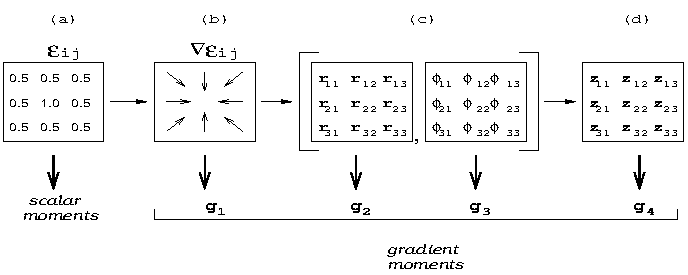
\includegraphics[width=\mylenfig]{./Figuras2/gpa.pdf}  
	\end{center}
	\vspace{4mm}	% acrescentar o espaçamento vertical apropriado entre a borda inferior da figura e a legenda ou a fonte quando não há legenda (o valor pode ser negativo para subir)
	\legenda{Exemplo de legenda curta.}	% legenda - opcional
	\label{figgpa1}
	\FONTE{\citeonline{lba/06}.}	% fonte consultada (elemento obrigatório, mesmo que seja produção do próprio autor)
\end{figure}

\begin{figure}[!h]
	\caption{Figura com título que ocupa mais de uma linha, alinhar as demais com a primeira
letra depois do hífen.}
%o ajuste do título é feito automaticamente pelo \LaTeX\ caso este ocupe mais de uma linha.}
	\vspace{6mm}	% acrescentar o espaçamento vertical apropriado entre o título e a borda superior da figura
	\begin{center}
    	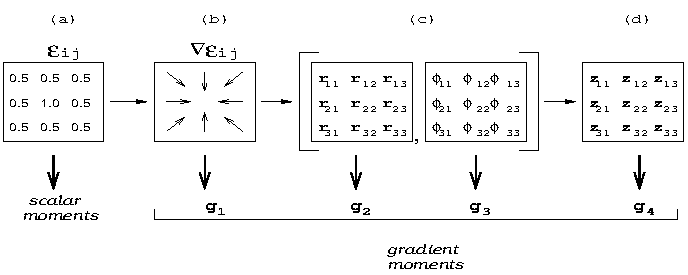
\includegraphics[width=\mylenfig]{./Figuras2/gpa.pdf}  
	\end{center}
	\vspace{4mm}	% acrescentar o espaçamento vertical apropriado entre a borda inferior da figura e a legenda ou a fonte quando não há legenda (o valor pode ser negativo para subir)
	\legenda{Exemplo de legenda que ocupa mais de uma linha, alinhar as demais com a primeira
letra da primeira linha.}	% legenda - opcional
%o \LaTeX\ alinha o texto automaticamente.
	\label{figgpa2}
	\FONTE{Se o texto da fonte for longo e ocupar mais de uma linha as demais ficam alinhadas
	com a palavra fonte. Adaptada de \citeonline{mauri:2003}.}	% fonte consultada (elemento obrigatório, mesmo que seja produção do próprio autor)
%o \LaTeX\ alinha o texto automaticamente.
\end{figure}

\clearpage
\section{Tabelas} 

\begin{table}[!ht]%[htbp] %opções de colocação da tabela no texto
  \begin{center}	% use sempre um ambiente para as tabelas
									% (opções: center (recomendado), flushright, flushleft)
									% NÃO USE \centering com TABELAS se houver \FONTE!	
  \caption{Exemplo de tabela, com fonte.}
    \begin{tabular}{l|l|c|c|r|r}
			\hline % desenha uma linha horizontal
				Campo 1 & Campo2 & Campo3 & Campo 4 & Campo5 & Campo6 \\
				Campo 1 & Campo2 & Campo3 & Campo 4 & Campo5 & Campo6 \\
				Campo 1 & Campo2 & Campo3 & Campo 4 & Campo5 & Campo6 \\				
			\hline % desenha uma linha horizontal
    \end{tabular}
    \end{center}
 \FONTE{Coloque a fonte de referência aqui, se houver.}
\end{table}

% \hhline{|--|} \multicolumn{2}{|c|}{continuação da página anterior} \\
% \hhline{|--|} \endhead % ate aqui eh definicao do "head" da pagina 
%   % dois em diante
% \hhline{|--|} \multicolumn{2}{|c|}{continua para próxima página} \\
% \hhline{|--|} \endfoot % ate aqui eh definicao do "foot" exceto ultima página
% \hhline{|b:=:=:b|} \endlastfoot % ate aqui eh definicao do "foot" 
%   % da ultima pagina

\begin{table}[hb]
\renewcommand{\baselinestretch}{1.4}% for tabular environment
\small
   \centering
   \caption{Exemplo de tabela, com fonte longa}
%   \label{\fullpaperid:table:1}% you must prefix your labels (here table:1) with the string \fullpaperid: (this will be important when combining all the full papers for the final book)
	\begin{center}
	   \begin{tabular}{lcc}
	       \hline% horizontal line
	       \itshape Parameter&
	           \itshape $\kappa$ Scaling&
	           \itshape $\kappa$, $\lambda$ Scaling\\*
	       \hline
	       Dimension&
	           $\kappa^{-1}$&
	           $\lambda^{-1}$\\*
	       Currant&
	           $\kappa^{-1}$&
	               $\lambda/\kappa^{2}$\\*
	       Dopant Concentration&
	           $\kappa$&
	           $\lambda2/\kappa$\\*
	       \hline
	   \end{tabular}
	\end{center}
    \renewcommand{\baselinestretch}{1.0}
    \FONTE{Coloque a fonte longa longa longa longa longa longa longa longa longa longa aqui, se houver.}
\end{table}

% Exemplos de 2 tabelas avançadas 

\begin{table}[ht!]
\caption{Outro exemplo de tabela}
%\label{\fullpaperid:table:2}
\begin{center}
\renewcommand{\baselinestretch}{1.2}% for tabular environment
\small
\begin{tabular}{cccccc}
\hline
   & \multirow{2}{22mm}{\renewcommand{\baselinestretch}{0.7}\small\centering Quantitative measures} & \multicolumn{4}{c}{Markers} \\ \cline{3-6}
   & & \multicolumn{1}{c}{RO} & \multicolumn{1}{c}{ASF} & \multicolumn{1}{c}{ISO} & \multicolumn{1}{c}{ADF} \\ \hline
   \multirow{3}{20mm}{\renewcommand{\baselinestretch}{0.7}\small\centering Test image scale 2}
& RMSE & 0.126 & 0.187 & 0.118 & 0.103 \\
& NMSE & 0.046 & 0.101 & 0.040 & 0.031 \\
& SSIM & 0.9981 & 0.9956 & 0.9984 & 0.9989 \\ \hline
   \multirow{3}{18mm}{\renewcommand{\baselinestretch}{0.7}\small\centering Cameraman scale 4}
& RMSE & 13.748 & 15.649 & 10.132 & 4.325 \\
& NMSE & 0.011 & 0.014 & 0.006 & 0.001 \\
& SSIM & 0.923 & 0.847 & 0.904 & 0.933 \\ \hline
   \multirow{3}{18mm}{\renewcommand{\baselinestretch}{0.7}\small\centering Cameraman scale 7}
& RMSE & 20.963 & 22.652 & 13.108 & 4.650 \\
& NMSE & 0.024 & 0.029 & 0.010 & 0.001 \\
& SSIM & 0.851 & 0.757 & 0.866 & 0.925 \\ \hline
   \multirow{3}{23mm}{\renewcommand{\baselinestretch}{1.2}\small\centering Crop of cameraman scale 7}
& RMSE & 30.914 & 31.943 & 17.831 & 2.870 \\
& NMSE & 0.053 & 0.057 & 0.018 & 0.001 \\
& SSIM & 0.831 & 0.772 & 0.891 & 0.983 \\ \hline
\end{tabular}
\end{center}
\end{table}

\begin{table}[ht!]
\caption{Mais um exemplo de tabela}
%\label{\fullpaperid:table:1}
\begin{center}
\renewcommand{\baselinestretch}{1.2}% for tabular environment
\small
\begin{tabular}{ccccc}
\hline
\multirow{4}{16mm}{\renewcommand{\baselinestretch}{0.7}\small\centering Leveling's Scale} & \multicolumn{4}{c}{Values for the scale relation of the four different type of markers} \\ \cline{2-5}
& \multirow{3}{29mm}{\renewcommand{\baselinestretch}{1}\small\centering Structure element's size $r$ for RO and ASF} & \multicolumn{2}{c}{Isotropic diffusion} & \multirow{3}{20mm}{\renewcommand{\baselinestretch}{1}\small\centering Anisotropic diffusion iterations $t$} \\ \cline{3-4}
& & \multirow{2}{23mm}{\renewcommand{\baselinestretch}{0.7}\small\centering Standard deviation $\sigma$} & \multirow{2}{12mm}{\renewcommand{\baselinestretch}{0.7}\small\centering Kernel size} & \\
& & & & \\ \hline
1 & 1 & 0.5 & $5 \times 5$ & 100 \\
2 & 2 & 1.0 & $7 \times 7$ & 200 \\
3 & 3 & 1.5 & $11 \times 11$ & 300 \\
4 & 4 & 2.0 & $13 \times 13$ & 400 \\
5 & 5 & 2.5 & $17 \times 17$ & 500 \\
6 & 6 & 3.0 & $19 \times 19$ & 600 \\
7 & 7 & 3.5 & $23 \times 23$ & 700 \\ \hline
\end{tabular}
\end{center}
\end{table} 

\setlongtables
\begin{longtable}[c]{c|c|c|c|c|c}
\caption{Exemplo de tabela longa que atravessa várias páginas.}\label{tab:longas}\\
\hline
\textbf{Campo1} & \textbf{Campo2} & \textbf{Campo3} & \textbf{Campo4} & \textbf{Campo5} & \textbf{Campo6} \\
\hline\hline
\endfirsthead
\caption[]{Continuação} \\
\hline
\textbf{Campo1} & \textbf{Campo2} & \textbf{Campo3} & \textbf{Campo4} & \textbf{Campo5} & \textbf{Campo6} \\
\hline\hline
\endhead
\hline\hline
\endlastfoot
\hline
\multicolumn{6}{r}{\captionlabelfont\captionsize(Continua)}\\
\endfoot


	campo1 & campo2 & campo3 & campo4 & campo5 & campo6 \\
	campo1 & campo2 & campo3 & campo4 & campo5 & campo6 \\
	campo1 & campo2 & campo3 & campo4 & campo5 & campo6 \\
	campo1 & campo2 & campo3 & campo4 & campo5 & campo6 \\
	campo1 & campo2 & campo3 & campo4 & campo5 & campo6 \\
	campo1 & campo2 & campo3 & campo4 & campo5 & campo6 \\
	campo1 & campo2 & campo3 & campo4 & campo5 & campo6 \\
	campo1 & campo2 & campo3 & campo4 & campo5 & campo6 \\
	campo1 & campo2 & campo3 & campo4 & campo5 & campo6 \\
	campo1 & campo2 & campo3 & campo4 & campo5 & campo6 \\
	campo1 & campo2 & campo3 & campo4 & campo5 & campo6 \\
	campo1 & campo2 & campo3 & campo4 & campo5 & campo6 \\
	campo1 & campo2 & campo3 & campo4 & campo5 & campo6 \\
	campo1 & campo2 & campo3 & campo4 & campo5 & campo6 \\
	campo1 & campo2 & campo3 & campo4 & campo5 & campo6 \\
	campo1 & campo2 & campo3 & campo4 & campo5 & campo6 \\
	campo1 & campo2 & campo3 & campo4 & campo5 & campo6 \\
	campo1 & campo2 & campo3 & campo4 & campo5 & campo6 \\
	campo1 & campo2 & campo3 & campo4 & campo5 & campo6 \\
	campo1 & campo2 & campo3 & campo4 & campo5 & campo6 \\
	campo1 & campo2 & campo3 & campo4 & campo5 & campo6 \\
	campo1 & campo2 & campo3 & campo4 & campo5 & campo6 \\
	campo1 & campo2 & campo3 & campo4 & campo5 & campo6 \\
	campo1 & campo2 & campo3 & campo4 & campo5 & campo6 \\
	campo1 & campo2 & campo3 & campo4 & campo5 & campo6 \\
	campo1 & campo2 & campo3 & campo4 & campo5 & campo6 \\
	campo1 & campo2 & campo3 & campo4 & campo5 & campo6 \\
	campo1 & campo2 & campo3 & campo4 & campo5 & campo6 \\
	campo1 & campo2 & campo3 & campo4 & campo5 & campo6 \\
	campo1 & campo2 & campo3 & campo4 & campo5 & campo6 \\
	campo1 & campo2 & campo3 & campo4 & campo5 & campo6 \\
	campo1 & campo2 & campo3 & campo4 & campo5 & campo6 \\
	campo1 & campo2 & campo3 & campo4 & campo5 & campo6 \\
	campo1 & campo2 & campo3 & campo4 & campo5 & campo6 \\
	campo1 & campo2 & campo3 & campo4 & campo5 & campo6 \\
	campo1 & campo2 & campo3 & campo4 & campo5 & campo6 \\
	campo1 & campo2 & campo3 & campo4 & campo5 & campo6 \\
	campo1 & campo2 & campo3 & campo4 & campo5 & campo6 \\
	campo1 & campo2 & campo3 & campo4 & campo5 & campo6 \\
	campo1 & campo2 & campo3 & campo4 & campo5 & campo6 \\
	campo1 & campo2 & campo3 & campo4 & campo5 & campo6 \\
	campo1 & campo2 & campo3 & campo4 & campo5 & campo6 \\
	campo1 & campo2 & campo3 & campo4 & campo5 & campo6 \\
	campo1 & campo2 & campo3 & campo4 & campo5 & campo6 \\
	campo1 & campo2 & campo3 & campo4 & campo5 & campo6 \\
	campo1 & campo2 & campo3 & campo4 & campo5 & campo6 \\
	campo1 & campo2 & campo3 & campo4 & campo5 & campo6 \\
	campo1 & campo2 & campo3 & campo4 & campo5 & campo6 \\
	campo1 & campo2 & campo3 & campo4 & campo5 & campo6 \\
	campo1 & campo2 & campo3 & campo4 & campo5 & campo6 \\
	campo1 & campo2 & campo3 & campo4 & campo5 & campo6 \\
	campo1 & campo2 & campo3 & campo4 & campo5 & campo6 \\
	campo1 & campo2 & campo3 & campo4 & campo5 & campo6 \\
	campo1 & campo2 & campo3 & campo4 & campo5 & campo6 \\
	campo1 & campo2 & campo3 & campo4 & campo5 & campo6 \\
	campo1 & campo2 & campo3 & campo4 & campo5 & campo6 \\
	campo1 & campo2 & campo3 & campo4 & campo5 & campo6 \\
	campo1 & campo2 & campo3 & campo4 & campo5 & campo6 \\
	campo1 & campo2 & campo3 & campo4 & campo5 & campo6 \\
	campo1 & campo2 & campo3 & campo4 & campo5 & campo6 \\
	campo1 & campo2 & campo3 & campo4 & campo5 & campo6 \\
	campo1 & campo2 & campo3 & campo4 & campo5 & campo6 \\
	campo1 & campo2 & campo3 & campo4 & campo5 & campo6 \\
	campo1 & campo2 & campo3 & campo4 & campo5 & campo6 \\
	campo1 & campo2 & campo3 & campo4 & campo5 & campo6 \\
	campo1 & campo2 & campo3 & campo4 & campo5 & campo6 \\
	campo1 & campo2 & campo3 & campo4 & campo5 & campo6 \\
	campo1 & campo2 & campo3 & campo4 & campo5 & campo6 \\
	campo1 & campo2 & campo3 & campo4 & campo5 & campo6 \\
	campo1 & campo2 & campo3 & campo4 & campo5 & campo6 \\
	campo1 & campo2 & campo3 & campo4 & campo5 & campo6 \\
	campo1 & campo2 & campo3 & campo4 & campo5 & campo6 \\
	campo1 & campo2 & campo3 & campo4 & campo5 & campo6 \\
\hline
\end{longtable}
% o comando \FONTE{} não pode ser usado neste caso
\vspace{-8mm}
\begin{center}
	Fonte: Referência a fonte da tabela.
\end{center}


A \autoref{tab:longa} é um exemplo de tabela no modo paisagem e que ocupa também várias páginas.

\setlongtables
\begin{landscape}
\begin{longtable}[c]{c|c|c|c|c|c|c|c|c|c}
\caption{Exemplo de tabela longa, em paisagem, que atravessa várias páginas.}\label{tab:longa}\\
\hline
\textbf{BOX1} & \textbf{BOX2} & \textbf{BOX3} & \textbf{BOX4} & \textbf{BOX5} & \textbf{BOX6} & \textbf{BOX7} & \textbf{BOX8} & \textbf{BOX9} & \textbf{BOX10} \\
\hline\hline
\endfirsthead
\caption[]{Conclusão}\\
\hline
\textbf{BOX1} & \textbf{BOX2} & \textbf{BOX3} & \textbf{BOX4} & \textbf{BOX5} & \textbf{BOX6} & \textbf{BOX7} & \textbf{BOX8} & \textbf{BOX9} & \textbf{BOX10} \\
\hline\hline
\endhead
\endlastfoot
\hline
\multicolumn{10}{r}{\captionlabelfont\captionsize(Continua)}\\
\endfoot
	
	BOX1 & BOX2 & BOX3 & BOX4 & BOX5 & BOX6 & BOX7 & BOX8 & BOX9 & BOX10 \\
	BOX1 & BOX2 & BOX3 & BOX4 & BOX5 & BOX6 & BOX7 & BOX8 & BOX9 & BOX10 \\
	BOX1 & BOX2 & BOX3 & BOX4 & BOX5 & BOX6 & BOX7 & BOX8 & BOX9 & BOX10 \\
	BOX1 & BOX2 & BOX3 & BOX4 & BOX5 & BOX6 &	BOX7 & BOX8 & BOX9 & BOX10 \\
	BOX1 & BOX2 & BOX3 & BOX4 & BOX5 & BOX6 &	BOX7 & BOX8 & BOX9 & BOX10 \\
	BOX1 & BOX2 & BOX3 & BOX4 & BOX5 & BOX6 &	BOX7 & BOX8 & BOX9 & BOX10 \\
	BOX1 & BOX2 & BOX3 & BOX4 & BOX5 & BOX6 &	BOX7 & BOX8 & BOX9 & BOX10 \\
	BOX1 & BOX2 & BOX3 & BOX4 & BOX5 & BOX6 &	BOX7 & BOX8 & BOX9 & BOX10 \\
	BOX1 & BOX2 & BOX3 & BOX4 & BOX5 & BOX6 &	BOX7 & BOX8 & BOX9 & BOX10 \\
	BOX1 & BOX2 & BOX3 & BOX4 & BOX5 & BOX6 &	BOX7 & BOX8 & BOX9 & BOX10 \\
	BOX1 & BOX2 & BOX3 & BOX4 & BOX5 & BOX6 & BOX7 & BOX8 & BOX9 & BOX10 \\
	BOX1 & BOX2 & BOX3 & BOX4 & BOX5 & BOX6 &	BOX7 & BOX8 & BOX9 & BOX10 \\
	BOX1 & BOX2 & BOX3 & BOX4 & BOX5 & BOX6 &	BOX7 & BOX8 & BOX9 & BOX10 \\
	BOX1 & BOX2 & BOX3 & BOX4 & BOX5 & BOX6 &	BOX7 & BOX8 & BOX9 & BOX10 \\
	BOX1 & BOX2 & BOX3 & BOX4 & BOX5 & BOX6 &	BOX7 & BOX8 & BOX9 & BOX10 \\
	BOX1 & BOX2 & BOX3 & BOX4 & BOX5 & BOX6 &	BOX7 & BOX8 & BOX9 & BOX10 \\
	BOX1 & BOX2 & BOX3 & BOX4 & BOX5 & BOX6 &	BOX7 & BOX8 & BOX9 & BOX10 \\
	BOX1 & BOX2 & BOX3 & BOX4 & BOX5 & BOX6 &	BOX7 & BOX8 & BOX9 & BOX10 \\
	BOX1 & BOX2 & BOX3 & BOX4 & BOX5 & BOX6 &	BOX7 & BOX8 & BOX9 & BOX10 \\                                 
	BOX1 & BOX2 & BOX3 & BOX4 & BOX5 & BOX6 &	BOX7 & BOX8 & BOX9 & BOX10 \\
	BOX1 & BOX2 & BOX3 & BOX4 & BOX5 & BOX6 &	BOX7 & BOX8 & BOX9 & BOX10 \\
	BOX1 & BOX2 & BOX3 & BOX4 & BOX5 & BOX6 &	BOX7 & BOX8 & BOX9 & BOX10 \\
	BOX1 & BOX2 & BOX3 & BOX4 & BOX5 & BOX6 &	BOX7 & BOX8 & BOX9 & BOX10 \\
	BOX1 & BOX2 & BOX3 & BOX4 & BOX5 & BOX6 &	BOX7 & BOX8 & BOX9 & BOX10 \\
	BOX1 & BOX2 & BOX3 & BOX4 & BOX5 & BOX6 &	BOX7 & BOX8 & BOX9 & BOX10 \\
	BOX1 & BOX2 & BOX3 & BOX4 & BOX5 & BOX6 &	BOX7 & BOX8 & BOX9 & BOX10 \\
	BOX1 & BOX2 & BOX3 & BOX4 & BOX5 & BOX6 &	BOX7 & BOX8 & BOX9 & BOX10 \\
	BOX1 & BOX2 & BOX3 & BOX4 & BOX5 & BOX6 &	BOX7 & BOX8 & BOX9 & BOX10 \\
\hline
\end{longtable}
\vspace{-8mm}
% o comando \FONTE{} não pode ser usado neste caso
\begin{center}
	Fonte: Referência a fonte da tabela.
\end{center}
\end{landscape}

%%%%%%%%%%%%%%%%%%%%%%%%%%%%%%%%%%%%%%%%%%%%%%%%%%%%%%%
%Anexo
%Este anexo foi incluido para explicar como incluir um anexo no estilo, não existia no original desta tese.
%%%%%%%%%%%%%%%%%%%%%%%%%%%%%%%%%%%%%%%%%%%%%%%%%%%%%%%%%%%%%%%%%%%%%%%%%%%%%%%%%
\renewcommand{\thechapter}{}%
\chapter{ANEXO C - TIPOS DE REFERÊNCIAS NO \LaTeX} %% Título do anexo sempre em maiúsculas.
\label{anexoC} %% Rótulo aplicado caso queira referir-se a este tópico em qualquer lugar do texto.
\renewcommand{\thechapter}{C}%

\begin{verbatim}

@BOOK{aacr2004, 
  title = {Cataloga{\c{c}}{\~a}o de recursos bibliogr{\'a}ficos 
  pelo {AACR2R} 2002}, 
  edition = {2},
  address = {Bras{\'i}lia},
  publisher = {Editora do Autor},
  author = {Antonia Motta Castro Memória Ribeiro},
  year = {2004}, 
  note = {v{\'a}rias p{\'a}gina{\c{c}}{\~o}es},
 }

@BOOK{rey93,
  title = {Planejar e redigir trabalhos cient\'ificos},
	subtitle = {teste de subtítulo},
  publisher = {Edgard Blücher},
  year = {1993},
  author = {Rey, L.},
  address = {S\~ao Paulo},
  pages = {318},
} 

@MISC{adobe00,
  title = {Adobe Acrobat 5.0.},
  year = {2000},
  note = {1 CD-ROM},
  address = {San Jose, CA},
  publisher = {Adobe Systems},
}


@ARTICLE{amaral98,
  author = {J. R. Amaral},
  title = {{INPE} estuda queda de meteorito na {A}maz{\^o}nia},
  journal = {Jornal Valeparaibano},
  year = {1998},
  month = {22 mar.},
  note = {Caderno 1, p. 12},
  address = {S{\~a}o Jos{\'e} dos Campos},}
}

@BOOK{assireu03,
  title = {Aplica{\c{c}}{\~a}o do operador de fragmenta{\c{c}}{\~a}o  
  assim{\'e}trica {(FA)} na caracteriza{\c{c}}{\~a}o de controles 
  geomorfol{\'o}gicos em reservat{\'o}rios hidrel{\'e}tricos},
  publisher = {INPE},
  year = {2003},
  author = {A. T. Assireu and E. M. L. M. Novo and J. A. Lorenzzetti 
  and C. Z.	F. Braga and I. B. T. Lima and J. L. Stech},
  address = {S{\~a}o Jos{\'e} dos Campos},
  note = {(INPE-9543-RPQ/737)},
  pages = {34},
}

@BOOK{assireu03e,
  title = {Aplica{\c{c}}{\~a}o do operador de fragmenta{\c{c}}{\~a}o 
  assim{\'e}trica {(FA)} na caracteriza{\c{c}}{\~a}o de controles 
  geomorfol{\'o}gicos em reservat{\'o}rios hidrel{\'e}tricos},
  publisher = {INPE},
  year = {2003},
  author = {A. T. Assireu and E. M. L. M. Novo and J. A. Lorenzzetti 
  and C. Z.	F. Braga and I. B. T. Lima and J. L. Stech},
  address = {S{\~a}o Jos{\'e} dos Campos},
  note = {(INPE-9543-RPQ/737)},
  pages = {34},
  url = {goto-/bol.com.br/mirian_cris/2003/01.31.11.23},
  urlaccessdate = {03 maio 2004},
}

@INCOLLECTION{aurelio86, 
  author = {Especializa{\c{c}}{\~a}o},
  editor = {Aur{\'e}lio Buarque Holanda Ferreira},  
  title = {Novo dicion{\'a}rio da l{\'\i}ngua portuguesa},
  publisher = {Nova Fronteira},
  year = {1986},
  address = {Rio de Janeiro}, 
  pages = {698},
  edition = {2},
}

@MANUAL{banon98,
  title = {Apresenta{\c{c}}{\~a}o e ilustra{\c{c}}{\~a}o de 
  uso de uma biblioteca digital},
  author = {G. F. Banon},
  address = {S{\~a}o Jos{\'e} dos Campos},
  year = {1998},
  note = {Palestra realizada no Instituto Nacional de Pesquisas 
  Espaciais (INPE),
	em 17 fev. 1998},
}

@MISC{barbosa70, 
  author = {O. Barbosa},
  title = {Projeto Leste do Tocantins/Oeste do Rio S{\~a}o Francisco},  
  publisher = {Companhia de Pesquisas de Recursos Minerais (CPRM)/
  Departamento Nacional de Produ{\c{c}}{\~a}o Mineral (DNPM)/(PROSPEC)},
  year = {1970},
  address = {Rio de Janeiro}, 
  pages = {170},
  note = {Conv{\^e}nio},
}

@THESIS{boggione03,
  address = {S{\~a}o Jos{\'e} dos Campos},
  author = {G. A. Boggione}, 
  note = {(INPE-10462-TDI/929)},
  pages = {2003. 160},
  school = {Instituto Nacional de Pesquisas Espaciais (INPE)},
  title = {Restaura{\c{c}}{\~a}o de imagens do sat{\'e}lite Landsat-7},
  type = {Disserta{\c{c}}{\~a}o (Mestrado em Sensoriamento Remoto)},
  year = {2003},
}

@ARTICLE{brasil74,
  title = {Decreto-lei nº 6129, de 6 de novembro de 1974. Disp\~oe 
  sobre a transforma{\c{c}}{\~a}o do Conselho Nacional de 
  Desenvolvimento Cient\'ifico e Tecnol\'ogico -- {CNPq}},
  journal = {Lex},
  year = {1974},
  volume = {38},
  pages = {1017-1018},
  month = {out./dez.},
  organization = {Brasil},
  section = {Legisla{\c{c}}{\~a}o Federal e Margin\'alia},
}

@ARTICLE{brasil04,
  title = {Portaria {CCIVIL} nº 388, de 15.04.2004. {D}esigna os 
  membros para compor a {C}omiss\~ao {E}xecutiva do {P}lano de 
  {A}{\c{c}}{\~a}o para a {P}reven{\c{c}}{\~a}o e {C}rontole do 
  {D}esmatamento na {A}maz\^onia {L}egal},
  year = {2004},
  organization = {Brasil},
  url = {http://www.mct.gov.br/legis/portarias/Minist.htm\#2004},
  urlaccessdate = {19 ago. 2004},
}

@MISC{brum99,
  author = {C. G. M. Brum},
  title = {Resistrador anal\'ogico usado para registrar o 
  ru\'ido c\'osmico},
  year = {1999},
  note = {1 fotografia},
  owner = {ePrint},
}

@BOOK{camara01,
  title = {Introdu{\c{c}}{\~a}o {\`a} ci{\^e}ncia da 
  geoinforma{\c{c}}{\~a}o},
  publisher = {INPE},
  year = {2001},
  editor = {G. C\^amara and C. Davis and A. M. V. Monteiro},
  address = {S{\~a}o Jos{\'e} dos Campos},
  pages = {344},
  url = {goto-/sid.inpe.br/sergio/2004/04.22.07.43},
  urlaccessdate = {22 de abr. 2004},
}

@BOOKLET{clima02,
  title = {{C}liman\'alise: {B}oletim de {M}onitoramento e 
  {A}n{\'a}lise {C}lim{\'a}tica},
  address = {S{\~a}o Jos{\'e} dos Campos: INPE},
  month = {jan.},
  year = {2002},
  number = {1},
  url = {http://www.cptec.inpe.br/products/climanalise/capa1.html},
  urlaccessdate = {3 maio 2004},
  volume = {17},
}

@BOOK{clima86,
  title = {Climan\'alise: Boletim de Monitoramento e 
  An\'alise Clim\'atica},
  publisher = {INPE},
  year = {1986},
  address = {S\~ao Jos\'e dos Campos},
  note = {Mensal},
}

@BOOKLET{clima96,
  title = {{C}liman\'alise: {B}oletim de {M}onitoramento e 
  {A}n{\'a}lise {C}lim{\'a}tica},
  address = {S{\~a}o Jos{\'e} dos Campos: INPE},
  month = {jan.},
  year = {1996},
  number = {1},
  pages = {53},
  volume = {11},
}

@BOOK{diller93,
  title = {\LaTeX\ by line},
  publisher = {John Wiley \& Sons},
  year = {1993},
  author = {Antoni Diller},
  address = {Chichester, West Sussex},
  isbn = {0-471-93471-2},
  pages = {291},
}

@INPROCEEDINGS{drummond03,
  author = {I. N. Drummond and L. Godo and S. A. Sandri},
  title = {Learning fuzzy systems with similarity relations},
  booktitle = {Proceedings...},
  year = {2003},
  pages = {516--523},
  address = {Istanbul},
  organization = {International Fuzzy Systems Association 
  World Congress},
  publisher = {ICI/IFSA},
  note = {(INPE-10533-PRE/6005)},
  conference-location = {Istanbul, Turkey},
  conference-number = {10},
  conference-year = {2003},
  isbn = {975-518-208-X},
  org-short = {IFSA},
}

@MISC{fepam92,
  title = {Mata {A}tl\^antica no Rio Grande do Sul},
  year = {1992},
  note = {1 Mapa. Escala 1:250.000},
  address = {Porto Alegre},
  org-short = {FEPAM},
  organization = {Funda{\c{c}}{\~a}o Estadual de Prote{\c{c}}{\~a}o 
  Ambiental Henrique Luis Roessler (FEPAM)},
  subtitle = {tombamento da {R}eserva da {B}iosfera},
  url = {http://www.fepam.rs.gov.br/programas/kfw.asp},
  urlaccessdate = {13 fev. 2002},
}

@ARTICLE{ferreira03,
  author = {R. N. Ferreira and T. M. Richenbach and D. L. Herdies 
  and L. M. V. Carvalho},
  title = {Variability of {S}outh {A}merican convective cloud systems and 
  tropospheric circulation during {J}anuary-{M}arch 1998 and 1999},
  journal = {Monthly Weather Review},
  year = {2003},
  volume = {131},
  pages = {961--973},
  number = {5},
  month = {May},
  note = {(INPE-9991-PRE/5551)},
}

@MISC{filme96,
  title = {Space: helping to complete the picture},
  year = {1996},
  note = {1 videocassete (15 min), VHS, son},
  address = {London},
  publisher = {BNSC},
}

@ARTICLE{formaggio01,
  author = {A. R. Formaggio and J. C. N. Epiphanio and M. D. Sim{\~o}es},
  title = {Radarsat backscattering from an agricultural scene},
  journal = {Pesquisa Agropecu{\'a}ria Brasileira},
  address = {Bras\'ilia},
  year = {2001},
  volume = {36},
  pages = {823--830},
  number = {5},
  url = {http://isi3.isiknowledge.com/portal.cgi?DestApp=WOS&Func=Frame},
  urlaccessdate = {3 maio 2004},
}
 
@BOOK{franca2004,
  title = {Manual para normaliza{\c{c}}{\~a}o de publica{\c{c}}{\~o}es 
  t\'ecnico-cient\'ificas},
  publisher = {UFMG},
  year = {2004},
  author = {Fran{\c{c}a} J\'unia Lessa  and  Vasconcellos Ana Cristina 
  and Magalh{\~a}es Maria Helena A. and  Borges Stella Maris},
  pages = {242},
  address = {Belo Horizonte},
}

@MISC{fsosma02a,
  title = {Atlas dos remanescentes florestais da {M}ata {A}tl{\^a}ntica; 
  per{\'i}odo 1995--2000},
  year = {2002a},
  note = {Cont{\'e}m 11 Mapas. (INPE-9694-PRP/238)},
  address = {S{\~a}o Jos{\'e} dos Campos},
  org-short = {FSOSMA},
  organization = {Funda{\c{c}}{\~a}o SOS Mata Atl\^antica 
  (FSOSMA) / 
  Instituto Nacional de Pesquisas	Espaciais (INPE)},
  pages = {47},
}

@MISC{fsosma02b,
  title = {Atlas dos remanescentes florestais da {M}ata 
  {A}tl{\^a}ntica; 
  per{\'i}odo	1995--2000},
  year = {2002b},
  note = {Cont{\'e}m 11 Mapas. (INPE-9694-PRP/238)},
  address = {S{\~a}o Jos{\'e} dos Campos},
  org-short = {FSOSMA},
  organization = {Funda{\c{c}}{\~a}o SOS Mata Atl\^antica 
  (FSOSMA)/ Instituto Nacional de Pesquisas 	Espaciais (INPE)},
  pages = {47},
  url = {goto-/sid.inpe.br/jeferson/2003/06.02.07.45},
  urlaccessdate = {3 maio 2004},
}

@BOOK{ibge93,
  title = {Normas de apresenta{\c{c}}{\~a}o tabular},
  publisher = {IBGE},
  year = {1993},
  address = {Rio de Janeiro},
  edition = {2},
  isbn = {85-240-0471-1},
  org-short = {IBGE},
  organization = {Instituto Brasileiro de Geografia e Estat\'istica
  (IBGE)},
  pages = {62},
}  

@MANUAL{inpe00,
  title = {Laborat{\'o}rio Associado de Combust{\~a}o e 
  Propuls{\~a}o(LCP)},
  organization = {Instituto Nacional de Pesquisas Espaciais 
  (INPE)},
  address = {Cachoeira Paulista},
  publisher = {INPE},
  year = {2000},
  note = {Folder},
  org-short = {INPE},
}

 @MISC{inpe87,
  title = {S{\~a}o Jos{\'e} dos Campos (SP)},
  year = {1987},
  note = {1 Mapa Topogr{\'a}fico. Escala 1:100.000},
  address = {S{\~a}o Jos{\'e} dos Campos},
  org-short = {INPE},
  organization = {Instituto Nacional de Pesquisas Espaciais (INPE)},
  subtitle = {atualiza{\c{c}}{\~a}o do uso da terra. {SF-23-YD-II-1 
  MI-2769/1}},
}


@MISC{inpe89,
  title = {{CBERS}},
  month = {jan.},
  year = {1989},
  note = {28 transpar{\^e}ncias. 25 x 20 cm},
  address = {S\~ao Jos\'e dos Campos},
  org-short = {INPE},
  organization = {Instituto Nacional de Pesquisas Espaciais (INPE)},
  publisher = {INPE},
}

@MISC{inpe95, 
  organization = {Instituto Nacional de Pesquisas Espaciais (INPE)},
  year = {1995},
  title = {Mem{\'o}ria {T}{\'e}cnico-{C}ient{\'i}fica do INPE},
  org-short = {INPE},
  subtitle = {biblioteca digital},
  url = {http://iris.sid.inpe.br:1905/col/sid.inpe.br/banon/2001/
  04.03.15.36.19/doc/mirror.cgi},
  urlaccessdate = {11 maio 2004},
} 
 
@MANUAL{inpedgi03,
  title = {Cat{\'a}logo CBERS 2},
  organization = {Instituto Nacional de Pesquisas Espaciais (INPE)},
  address = {S{\~a}o Jos{\'e} dos Campos},
  year = {2004},
  org-short = {INPE},
  url = {http://www.dgi.inpe.br},
  urlaccessdate = {03 maio 2004},
}

@MISC{inpedgi04,
  title = {Imagem da cidade de S{\~a}o Jos{\'e} dos Campos},
  year = {2004},
  note = {Cachoeira Paulista, 2000. 1 imagem de sat{\'e}lite. CBERS 2 / 
  Sensor 	CCD. 30 jan. 2004. Base 153 / Ponto: 126, Composi{\c{c}}{\~a}o 
  RGB, bandas	4, 3, 2},
  organization = {Instituto Nacional de Pesquisas Espaciais. Divis{\~a}o de 
  Gera{\c {c}}{\~a}o de Imagens (INPE.DGI)},
  org-short = {INPE.DGI},
}

@MISC{inpedgi05,
  title = {Imagem da cidade de S{\~a}o Jos{\'e} dos Campos},
  year = {2004},
  note = {Cachoeira Paulista, 2000. 1 imagem de sat{\'e}lite. CBERS 1 / 
  Sensor CCD -- Composi{\c{c}}{\~a}o RGB, bandas 4, 3, 2, Base 153 / 
  Ponto: 126},
  organization = {Instituto Nacional de Pesquisas Espaciais. 
  {Divis{\~a}o de Gera{\c {c}}{\~a}o de Imagens (INPE-DGI)}},
  org-short = {INPE-DGI},
  url = {http://www.dgi.inpe.br/html/gal-2.htm},
  urlaccessdate = {20 abr. 2004},
}

@PATENT{inpep95,
  organization = {INSTITUTO NACIONAL DE PESQUISAS ESPACIAIS}, 
  howpublished = {Vladimir Jesus Trava-Airoldi and Evaldo Jose Corat 
  and Edson Del Bosco and Marcia Carneiro Valera and Angel Fidel 
  Pi{\~n}a and Victor Baranauskas and N{\'e}lia Ferreira Leite},
  year = {1995},
  title = {Brocas para uso odontol{\'o}gico ou uso correlato de desgaste ou 
  perfura{\c{c}}{\~a}o revestidas com diamante obtido com as t{\'e}cnicas 
  qu{\'í}micas de crescimento a partir da Fase 
  Vapor-CVD (Chemical Vapor Deposition)},
  note = {21 fev. 1995, 8 out. 2002},
  number = {BR, n. PI 9500865-9},
}

@PATENT {Scha84
  organization = {Santrade Limited},
  year = {1985},
  furtherresp = {Schachner H.},
  title = {Body with superhard coating},
  number = {4,734,339},
  howpublished = {Mar. 29, 1988 and Jun. 24, 1985},
}

@MISC{gomes98,
  title = {Elei{\c{c}}{\~a}o}, 
  year = {1998},
  note = {Entrevistador: M{\'a}rcio Manzi Alvarenga. 
  Uberl{\^a}ndia: Funda{\c{c}}{\~a}o R{\'a}dio e Televis{\~a}o 
  Educativa de Uberl{\^a}ndia, 30 mar. 1998. Entrevista 
  concedida ao programa de televisão "Acontece o seguinte".},
  author = {C Gomes}, 
  subtitle = {poss{\'i}vel candidatura},
}

@BOOK{goossens94,
  title = {The \LaTeX\ companion},
  publisher = {Addison-Wesley},
  year = {1994},
  author = {Michel Goossens and Frank Mittelbach and 
  Alexander Samarin},
  address = {Reading, Massachusetts},
  bibliograpy = {yes},
  index = {yes},
  isbn = {0-201-54199-8},
  pages = {530},
}

@ARTICLE{jeon92,
  author = {B. Jeon and D. A. Landgrebe},
  title = {Classification with spatio-temporal interpixel 
  class dependency 
  contexts},
  journal = {IEEE Transactions on Geoscience and Remote 
  Sensing},
  year = {1992},
  volume = {30},
  pages = {664-672},
  number = {4},
  month = {July},
  note = {Special issue on the 1991 International 
  Geoscience and Remote 
  Sensing
	Symposium (IGARSS'91)},
}

@ARTICLE{jereissati98,
  author = {T. Jereissati},
  title = {Cuidado com o já ganhou},
  journal = {Veja},
  year = {1998},
  address = {S{\~a}o Paulo},
  volume = {31}, 
  pages = {9--11},
  number = {11},
  month =  mar,
  note = {Entrevista concedida a Ernesto Bernardes},
}

@UNPUBLISHED{kishore,
  author = {Ram Kishore and A. K. Mishra},
  year = {},
  title = {Algebra of orthofermions and equivalence of their 
thermodynamics to the infinite U Hubbard model},
  note  = {Aceito pela revista Physica B. 
  Acesso em: 21 jun. 2006.},
}   
        
@INCOLLECTION{kirchhoff91,
  author = {V. W. J. H. Kirchhoff},
  title = {Composi{\c{c}}{\~a}o, estrutura, 
  press{\~a}o e densidade},
  booktitle = {Introdu{\c{c}}{\~a}o {\`a} 
  geof{\'\i}sica espacial},
  publisher = {INPE},
  year = {2001},
  editor = {V. W. J. H. Kirchhoff},
  chapter = {3},
  pages = {31--42},
  address = {S{\~a}o Paulo},
  note = {149 p.},
}

@BOOK{kotait81,
  title = {Editora{\c{c}}{\~a}o cient{\'i}fica},
  publisher = {{\'A}tica},
  year = {1981},
  author = {Ivani Kotait},
  address = {S\~ao Paulo},
  pages = {118},
}

@MANUAL{man90,
  title = {Manual de normas para publica{\c{c}}{\~o}es 
  t{\'e}cnico-cient{\'i}ficas},
  organization = {Instituto Nacional de Pesquisas 
  Espaciais (INPE)},
  org-short = {INPE},
  address = {S{\~a}o Jos{\'e} dos Campos},
  publisher = {INPE},
  year = {1990},
  pages = {133},
  note = {(INPE-5116-MAN/001)},
}

@BOOK{massago04, 
  title = {Um Curso de latex via exemplos},
  publisher = {UFSCAR}, 
  year = {2002},
  author = {Sadao Massago},
  address = {S{\~a}o Paulo},
  url = {http://www2.dm.ufscar.br/~sadao/curso/latex/},
  urlaccessdate = {25 maio 2006},
}


@INCOLLECTION{medeiros01,
  author = {J. S. Medeiros and G. C{\^a}mara},
  title = {Geoprocessamento para projetos ambientais},
  booktitle = {Introdu{\c{c}}{\~a}o {\`a} ci{\^e}ncia da 
  geoinforma{\c{c}}{\~a}o},
  publisher = {INPE},
  year = {2001},
  editor = {G. C\^amara and C. Davis and A. M. V. Monteiro},
  address = {S{\~a}o Jos{\'e} dos Campos},
  note = {(INPE-8568-PRE/4312)},
  url = {goto-/sid.inpe.br/sergio/2004/04.19.15.08},
  urlaccessdate = {23 abr. 2004},
}

@MANUAL{NBR6021:1994a,
  title = {{NBR} 6021},
  organization = {Associa{\c{c}}{\~a}o Brasileira de 
  Normas T{\'e}cnicas (ABNT)},
  address = {Rio de Janeiro},
  month = oct,
  year = {1994a},
  org-short = {ABNT},
  pages = {3},
  subtitle = {Apresenta{\c{c}}{\~a}o de peri\'odicos},
}

@MANUAL{NBR6022:1994b,
  title = {{NBR} 6022},
  organization = {Associa{\c{c}}{\~a}o Brasileira de 
  Normas T{\'e}cnicas (ABNT)},
  address = {Rio de Janeiro},
  month = aug,
  year = {1994b},
  org-short = {ABNT},
  pages = {2},
  subtitle = {Apresenta{\c{c}}{\~a}o de artigos em 
  publica{\c{c}{\~o}es} 
  peri\'odicas},
}

@MANUAL{NBR6023:2002b,
  title = {{NBR} 6023},
  organization = {Associa{\c{c}}{\~a}o Brasileira de Normas 
  T{\'e}cnicas (ABNT)},
  address = {Rio de Janeiro},
  month = aug,
  year = {2002b},
  org-short = {ABNT},
  pages = {24},
  subtitle = {Informa{\c{c}}{\~a}o e documenta{\c{c}}{\~a}o: 
  refer\^encias: 
  elabora{\c{c}}{\~a}o},
}

@MANUAL{NBR6024:1989c,
  title = {{NBR} 6024},
  organization = {Associa{\c{c}}{\~a}o Brasileira de 
  Normas T{\'e}cnicas (ABNT)},
  address = {Rio de Janeiro},
  month = aug,
  year = {1989c},
  org-short = {ABNT},
  pages = {2},
  subtitle = {Numera{\c{c}}{\~a}o progressiva das 
  se{\c{c}}{\~o}es de um documento},  
} 

@MANUAL{NBR6026:1994c,
  title = {{NBR} 6026},
  organization = {Associa{\c{c}}{\~a}o Brasileira de 
  Normas T{\'e}cnicas (ABNT)},
  address = {Rio de Janeiro},
  month = mar,
  year = {1994c},
  org-short = {ABNT},
  pages = {2},
  subtitle = {Legenda bibliogr{\'a}fica},
}

@MANUAL{NBR6027:1989b,
  title = {{NBR} 6027},
  organization = {Associa{\c{c}}{\~a}o Brasileira de 
  Normas T{\'e}cnicas (ABNT)},
  address = {Rio de Janeiro},
  month = aug,
  year = {1989b},
  org-short = {ABNT},
  pages = {2},
  subtitle = {Sum{\'a}rio},
}

@MANUAL{NBR6028:1990,
  title = {{NBR} 6028},
  organization = {Associa{\c{c}}{\~a}o Brasileira de 
  Normas T{\'e}cnicas (ABNT)},
  address = {Rio de Janeiro},
  month = may,
  year = {1990},
  org-short = {ABNT},
  pages = {3},
  subtitle = {Resumos},
}

@MANUAL{NBR6029:2005b,
  title = {{NBR} 6029},
  organization = {Associa{\c{c}}{\~a}o Brasileira de 
  Normas T{\'e}cnicas (ABNT)},
  address = {Rio de Janeiro},
  month = sep,
  year = {2005b},
  org-short = {ABNT},
  pages = {9},
  subtitle = {Informa{\c{c}}{\~a}o e documenta{\c{c}}{\~a}o: 
  livros e folhetos: 
  Apresenta{\c{c}}{\~a}o},
}

@MANUAL{NBR6032:1989,
  title = {{NBR} 6032},
  organization = {Associa{\c{c}}{\~a}o Brasileira de 
  Normas T{\'e}cnicas (ABNT)},
  address = {Rio de Janeiro},
  month = aug,
  year = {1989},
  org-short = {ABNT},
  pages = {14},
  subtitle = {Abrevia{\c{c}}{\~o}es de T{\'i}tulos de 
  peri{\'o}dicos e 
  publica{\c{c}}{\~o}es 
  seriadas},
}

@MANUAL{NBR6033:1989,
  title = {{NBR} 6033},
  organization = {Associa{\c{c}}{\~a}o Brasileira de 
  Normas T{\'e}cnicas (ABNT)},
  address = {Rio de Janeiro},
  month = aug,
  year = {1989},
  org-short = {ABNT},
  pages = {5},
  subtitle = {Ordem alfab{\'e}tica},
}

@MANUAL{NBR6034:1989d,
  title = {{NBR} 6034},
  organization = {Associa{\c{c}}{\~a}o Brasileira de 
  Normas T{\'e}cnicas (ABNT)},
  address = {Rio de Janeiro},
  month = aug,
  year = {1989d},
  org-short = {ABNT},
  pages = {3},
  subtitle = {Prepara{\c{c}}{\~a}o de {\'i}ndice de publica{\c{c}}{\~o}es},
}

@MANUAL{NBR10520:2002a,
  title = {{NBR} 10520},
  organization = {Associa{\c{c}}{\~a}o Brasileira de 
  Normas T{\'e}cnicas (ABNT)},
  address = {Rio de Janeiro},
  month = aug,
  year = {2002a},
  org-short = {ABNT},
  pages = {7},
  subtitle = {Informa{\c{c}}{\~a}o e documenta{\c{c}}{\~a}o: 
  apresenta{\c{c}}{\~a}o de 
  cita{\c{c}}{\~o}es em documentos},
}

@MANUAL{NBR10521:1988,
  title = {{NBR} 10521},
  organization = {Associa{\c{c}}{\~a}o Brasileira de 
  Normas T{\'e}cnicas (ABNT)},
  address = {Rio de Janeiro},
  month = oct,
  year = {1988},
  org-short = {ABNT},
  pages = {2},
  subtitle = {Numera{\c{c}}{\~a}o internacional para livro: isbn},
}

@MANUAL{NBR10719:1989a,
  title = {{NBR} 10719},
  organization = {Associa{\c{c}}{\~a}o Brasileira de 
  Normas T{\'e}cnicas (ABNT)},
  address = {Rio de Janeiro},
  month = aug,
  org-short = {ABNT},
  pages = {17},
  subtitle = {Apresenta{\c{c}}{\~a}o de relat{\'o}rios  
  t{\'e}cnico-cient{\'i}ficos},
  year = {1989a},
}

@MANUAL{NBR12256:1992,
  title = {{NBR} 12256},
  organization = {Associa{\c{c}}{\~a}o Brasileira de 
  Normas T{\'e}cnicas (ABNT)},
  address = {Rio de Janeiro},
  month = apr,
  year = {1992},
  org-short = {ABNT},
  pages = {4},
  subtitle = {Apresenta{\c{c}}{\~a}o de originais},
}

@MANUAL{NBR14724:2005a,
  title = {{NBR} 14724},
  organization = {Associa{\c{c}}{\~a}o Brasileira de 
  Normas T{\'e}cnicas (ABNT)},
  address = {Rio de Janeiro},
  month = jan,
  year = {2005a},
  org-short = {ABNT},
  pages = {9},
  subtitle = {Informa{\c{c}}{\~a}o e documenta{\c{c}}{\~a}o: 
  trabalhos acad{\^e}micos: apresenta{\c{c}}{\~a}o},
}

@TECHREPORT{mauri:2003,
   author = {Instituto Nacional de Pesquisas (INPE)}, 
   year = {2003},
   title = {Resolu{\c{c}}{\~a}o do problema de programa{\c{c}}{\~a}o 
   de tripula{\c{c}}{\~o}es de um sistema de transporte p{\'u}blico via 
   simulated annealing},
   address = {Ouro Preto},
   organization = {Departamento de Ci{\^e}ncia da Computa{\c{c}}{\~a}o{-} 
   Universidade Federal de Ouro Preto},
   url = {http://www.decom.ufop.br/prof/marcone/Orientacoes/
   PPTviaSimulatedAnnealing.pdf},
   urlaccessdate  = {28 ago. 2006},   
   note = { 98p. Relat{\'orio t{\'e}cnico}},
}


@THESIS{padua04,
  address = {S{\~a}o Jos{\'e} dos Campos},
  author = {Marcelo Banik  P\'adua},
  pages = {2004. 162},
  note = {(INPE-12565-TDI/1004)},
  school = {Instituto Nacional de Pesquisas Espaciais (INPE)},
  title = {Estudo da indu{\c{c}}{\~a}o eletromagn{\'e}tica na 
  caracteriza{\c{c}}{\~a}o de estruturas profundas sob a borda sul do
  cr{\'a}ton de S{\~a}o Francisco},
  type = {Tese (Doutorado em Geof{\'i}sica)},
  url = {http://mtc-m16.sid.inpe.br:80/rep/sid.inpe.br/jeferson/
  2005/02.15.14.39},
  urlaccessdate = {22 ago. 2005}, 
  year = {2004},
}

@MISC{padua05,
  author = {Irani In{\'a}cio Cordeiro P\'adua},
  title = {Estilo TDIINPE LaTeX},
  year = {2005},
  note = {58 transparências}, 
  address = {S{\~a}o Jos{\'e} dos Campos},
  publisher = {INPE},
  subtitle = {Curso de editora{\c{c}}{\~a}o eletr{\^o}nica e 
publica{\c{c}}{\~a}o t{\'e}cnico-cient{\'i}fica},
  url = {http://ePrint.sid.inpe.br:1905/rep/sid.inpe.br/ePrint@1905/
  2005/10.26.13.54},
  urlaccessdate = {19 jun. 2006},
}

@MISC{parc96, 
  title = {Parc-nov.xls},
  organization = {Instituto Nacional de Pesquisas Espaciais (INPE)},
  address = {S{\~a}o Jos{\'e} dos Campos},
  year = {1996},
  note = {tabela de par{\^a}metros dendrom{\'e}tricos para estimativa de 
  biomassa.  1 disquete. 
  3.5 pol. 120832 caracteres. Excel.},
}

@BOOK{prado01,
  title = {Trajet{\'o}rias espaciais e manobras assistidas por gravidade},
  publisher = {INPE},
  year = {2001},
  author = {F. A. B. A. Prado},
  address = {S{\~a}o Jos{\'e} dos Campos},
  pages = {169},
}

@MISC{radam83,
  title = {Folhas {SC}. 24/25 Aracaj{\'u}/Sergipe}, 
  subtitle = {geologia, geomorfologia, pedologia, vegeta{\c{c}}{\~a}o e 
  uso potencial da terra}, 
  year = {1983},
  organization = {PROJETO RADAMBRASIL},
  address = {Rio de Janeiro},
  publisher = {IBGE},
  note = {5 mapas col. (Levantamento de Recursos Naturais, 30)},
  pages = {856},
 
}

@ARTICLE{raun95,
  author = {W. R. Raun and H. J. Barreto},
  title = {Regional maize grain response to applied phosphorus in 
  {C}entral	{A}merica},
  journal = {Agronomy Journal},
  year = {1995},
  volume = {87},
  pages = {208-213},
  number = {2},
  month = {Mar.},
  note = {Resumo em \textbf{Abstracts in Tropical Agriculture}, v. 20, 
  n. 12, p. 100, Dec. 1995},
}

@MANUAL{rca73,
  title = {Silicon transistor for 200-watt quasi-complementary symmetry 
  audio	amplifiers with parallel output transistor},
  organization = {Radio Corporation of America (RCA)},
  address = {Somerville, NJ},
  year = {1973},
  note = {Cat\'alogo},
  org-short = {RCA},
}

@BOOK{rey93,
  title = {Planejar e redigir trabalhos cient\'ificos},
	publisher = {Edgard Blücher},
  year = {1993},
  author = {Rey, L.},
  address = {S\~ao Paulo},
  pages = {318},
} 
  
@INPROCEEDINGS{rocha2005,
 author = {Elizabeth Rocha  and  Maria Feitosa Barros and Rafael 
 Silva Cruz and Carla Bernadete Madureira},
 title = {Uso de modelos digitais de eleva{\c{c}}{\~a}o de 
imagens de Radar para extra{\c{c}}{\~a}o de fei{\c{c}}{\~o}es 
topogr{\'a}ficas {-}um estudo de caso Maci{\c{c}}o da Tijuca, vertente 
Ba{\'i}a da Guanabara},
 booktitle = {Anais...},
 year = {2005}, 
 pages = {4469--4472}, 
 publisher = {{INPE}}, 
 address = {S{\~a}o Jos{\'e} dos Campos},
 organization = {Simp{\'o}sio Brasileiro de Sensoriamento Remoto},
 conference-location = {Goi{\^a}nia},
 conference-number = {12},
 conference-year = {2005},
 url = {http://marte.dpi.inpe.br:80/rep/ltid.inpe.br/sbsr/2004/
 11.20.11.59},
 urlacessdate = {12 jun. 2006},   
}
 
@MISC{rudorff04,
  author = { B. F. T. Rudorff},
  title = {Autoriza{\c{c}}{\~a}o para c{\'o}pia de publica{\c{c}}{\~a}o},
  year = {2004},
  note = {[mensagem pessoal].Mensagem recebida por \url{pubtc@sid.inpe.br} 
  em 19 abr. 2004},
}

@BOOK{saty04,
  title = {Rudimentos de meteorologia dinâmica},
  publisher = {INPE},
  year = {2004},
  author = {Satyamurty, P.},
  address = {S{\~a}o Jos{\'e} dos Campos},
  isbn = {85-17-00019-6},
  note = {(INPE-11437-RPQ/769)},
  pages = {154},
  url = {http://mtc-m16.sid.inpe.br/rep-/sid.inpe.br/marciana/2004/
  10.07.14.05},
  urlaccessdate = {02 out. 2006},
}

@INPROCEEDINGS{shima03,
  author = {Yosio Edemir Shimabukuro and Tomoaki Miura and Alfredo Huete 
  and  Egidio Arai and Fernando Del Bon Esp\'irito-Santo and Marcelo 
  Lopes Latorre},
  title = {An{\'a}lise dos dados hiperespectrais do {EO}-1 obtidos 
  sobre a {F}loresta {N}acional de {T}apaj{\'o}s no estado do {P}ar{\'a}},
  booktitle = {Anais...},
  year = {2003},
  pages = {1099--1106},
  publisher = {INPE},
  address = {S{\~a}o Jos{\'e} dos Campos},
  organization = {Simp{\'o}sio Brasileiro de Sensoriamento Remoto},
  note = {1 CD-ROM},
  conference-location = {Belo Horizonte},
  conference-number = {11},
  conference-year = {2003},
}

@INPROCEEDINGS{shima03e,
  author = {Yosio Edemir Shimabukuro and Tomoaki Miura and 
  Alfredo Huete and  Egidio Arai and Fernando Del Bon Esp{\'i}rito-Santo 
  and Marcelo Lopes Latorre},
  title = {An{\'a}lise dos dados hiperespectrais do {EO}-1 obtidos 
  sobre a   {F}loresta {N}acional de {T}apaj{\'o}s no estado do {P}ar{\'a}},
  booktitle = {Anais...},
  year = {2003},
  pages = {1099--1106},
  publisher = {INPE},
  address = {S{\~a}o Jos{\'e} dos Campos},
  organization = {Simp{\'o}sio Brasileiro de Sensoriamento Remoto},
  conference-location = {Belo Horizonte},
  conference-number = {11},
  conference-year = {2003},
  url = {goto-/ltid.inpe.br/sbsr/2002/11.17.13.39},
  urlaccessdate = {22 abr. 2004},
}

@INCOLLECTION{souza01,
  author = {M. L. O. Souza},
  title = {Sistemas de controle de atitude e de {\'o}rbita},
  booktitle = {Fundamentos de tecnologia espacial},
  publisher = {INPE},
  year = {2001},
  editor = {A. F. B. A. Prado and H. K. Kuga},
  chapter = {10},
  pages = {133--137},
  address = {S{\~a}o Jos{\'e} dos Campos},
}

@ARTICLE{taylor96,
  author = {D. Taylor},
  title = {{WWW} weatherfax images},
  journal = {{YACHT-L}},
  year = {1996},
  url = {listserv@hearn.bitnet},
  urlaccessdate = {17 Apr. 1996},
}

@BOOK{tierno2006,   
  title = {Ferramentas do word de apoio para utiliza{\c{c}}{\~a}o do 
  TDIINPE.dot},
  publisher = {INPE},  
  year = {2006},  
  author = {Maria Ros{\'a}rio Giffoni Tierno}, 
  address = {S{\~a}o Jos{\'e} dos Campos},   
  pages = {50},  
  url = {http://ePrint.sid.inpe.br:1905/rep/sid.inpe.br/
  ePrint@1905/2006/}, 
  urlaccessdate = {jul. 2006},
}

@MANUAL{tourrilhes2001,
  author = {Jean Tourrilhes},
  year = {2001},
  title = {A bit More about the technologies involved},
  subtitle = {Information and documentation},
  url = {http://www.hpl.hp.com/personal/Jean_Tourrilhes/Linux/Linux.
  Wireless.Overview.html},
  urlaccessdate = {15 jun. 2005},
}

%transparência
 @MISC{traina2002,
  author ={Agma Juici Machado Traina and Traina, Junior, Caetano}
  title = {Como escrever artigos cient{\'i}ficos},
  publisher = {UFSCAR},
  year = {2002},
  note = {27 transparências},
  url = {http://gbdi.icmc.usp.br/disciplinas/sce-5845/ComoEscrever
  /Single.html},
  urlaccessdate = {25 maio 2006},
}

 @INCOLLECTION{venancio84,
  author = {Alberto {VEN{\^A}NCIO FILHO}},
  title =  {Constituição de 1934},
  booktitle = {Dicion{\'a}rio hist{\'o}rico biogr{\'a}fico brasileiro 
  1930-1983},
  editor = {I. Beloch  and  A. A. Abreu},
  publisher = {FGV, CPDOC : FINEP}, 
  year = {1984},
  address = {Rio de Janeiro}, 
  pages = {913-914},
  volume = {2},
}  

@INCOLLECTION{camposvelho97,
  author = {Haroldo Fraga, Campos Velho},
  title =  {Constituição de 1934},
  booktitle = {Dicion{\'a}rio hist{\'o}rico biogr{\'a}fico brasileiro 
  1930-1983},
  editor = {I. Beloch  and  A. A. Abreu},
  publisher = {FGV, CPDOC : FINEP}, 
  year = {1997},
  address = {Rio de Janeiro}, 
  pages = {913-914},
  volume = {2},
}  

%Este é um exemplo de capítulo de livro 

@INCOLLECTION{sousa:2004,
  author = {SOUSA, F.L. and RAMOS, F.M. and GALSKI, R.L. and MURAOKA, I.},
  title = {Generalized extremal optimization: a new meta-heuristic inspired by a model of natural evolution},
  booktitle = {Recent developments in biologically inspired computing},
  publisher = {Idea Group Inc.},
  year = {2004},
  editor = {Leandro N. de Castro and Fernando J. Von Zuben},
  chapter = {},
  pages = {41--60},
  address = {Hershey PA},
}

 @ARTICLE{dias,
 author = {Silva, Dias, M. A. F.},
 title = { Sistemas de Mesoescala e previs{\~a}o de tempo a curto prazo},
 journal = {Revista Brasileira de Meteorologia},
 volume = {2},
 pages = {133-150},
 year = {1987},
}

%Este exemplo segundo uma aluna fica com et al nos autores 

@ARTICLE{Oost02, 
 author = {W.A. Oost and G.J Komen and C.M.J. Jacobs and C.V. Oort},
 title = {New Evidence For a Relation Between Wind Stress and  Wave age 
 from Measurements During Asgamage},
 journal = {Boundary Layer Meteorology},
 year = {2002},
 volume = {103},
 pages = {409-438}
}

%Este é um exemplo de título de tese com subtítulo

@THESIS{leite04,
 address = {Maceió},
 author = {C.C. Leite},
 school = {Universidade Federal de Alagoas (UFAL)},
 title = {Características da {C}amada {L}imite {C}onvectiva durante a 
 transi{\c{c}}{\~a}o da  esta{\c{c}}{\~a}o seca para chuvosa na {A}maz\^onia (2002)},
 subtitle = {{C}omparação {F}loresta/{P}astagem ({DRY TO WET AMC}/{LBA})},
 type = {Dissertação (Mestrado em Meteorologia)},
 year = {2004},
}


%Este é um exemplo de capítulo de livro, onde foi adicionado o campo nota, 
%para indicar a série 

 @INCOLLECTION{athanassoula01,
 author = {Evangelia Athanassoula},
 title = {Secular evolution of disc galaxies and of their components},
 booktitle = {Mapping the galaxy and nearby galaxies},
 publisher = {Springer},
 year = {2008},
 editor = {Keiichi Wada and Françoise Combes},
 address = {New York},
 pages = {47--54},
 note = {Astrophysics and Space Science Proceedings},
}

%Este é um exemplo para decreto publicado em coletânea, 
%criado pelo Estado de São Paulo

 @ARTICLE{saopaulo98,
 organization = {S{\~a}o Paulo {(Estado)}},  
 title = {Decreto nº 42.822, de 20 de janeiro de 1998},
 journal = {Lex:},	
 section = {colet\^anea de legisla{\c{c}}{\~a}o e jurisprud\^encia},
 year = {1998},
 volume = {62},
 number = {3},
 pages = {217-220},
 address = {S{\~a}o Paulo },
}

%Este é um exemplo para título contendo aspas 
 @THESIS{mattos/06,
 address = {S{\~a}o Jos{\'e} dos Campos},
 author = {Mattos, Jo{\~a}o Gerd Zell},
 note = {(INPE-14794-TDI/1237)},
 pages = {2006. 129},
 school = {Instituto Nacional de Pesquisas Espaciais (INPE)},
 title = {Sensibilidade do uso de "Pseudo-temps" na  assimila{\c{c}}{\~a}o 
 de dados do modelo de  circula{\c{c}}{\~a}o geral atmosf{\'e}rica do CPTEC/COLA},
 type = {Tese (Doutorado em Meteorologia)},
 year = {2006},              
 url = {http://urlib.net/sid.inpe.br/mtc-m17@80/2007/02.15.17.37},
 urlaccessdate = {12 abr. 2011},
}
 
%Este é um exemplo de título com fórmulas e sigla
 @ARTICLE{chedin:2003,
 author = {A. Chedin and S. Serrar and N.A. Scott and C. Crevoisier and R. Armante},
 title = {First global measurement of midtropospheric {CO}$_2$ 
         from {NOAA} polar	satellites: tropical zone},
 journal = {J. Geophys. Res.},
 volume = {108 (D18)},
 pages = {13 pp.},
 year =  {2003},
 note =  {4581, doi:10.1029/2003JD003439},
}

%Este é um exemplo de relatório técnico cujo título tem subtítulo e 
% cujo autor é uma entidade

@TECHREPORT{IPCC:2001,
   year = {2001},
   title = {Climate change 2001},
	 subtitle = {the physical science basis. contribution of working group I
	 to the third assessment
   report of the intergovernmental panel on climate change},
   address = {Cambridge, United Kingdom},
   organization = {Intergovernmental Panel on Climate Change (IPCC)},
   url = {http://www.grida.no/publications/other/ipcc_tar/},
   urlaccessdate  = { },  
   note = {98p. Relat{\'orio t{\'e}cnico}},
}

%Este é um exemplo de livro com subtítulo 

@BOOK{Beale:90,
  author = {Beale, R.; Jackson, T.},
  title =   {Neural computing},
	subtitle = {an introduction},
  edition =  {},
  address =  {New York, NY},
  publisher = {Adam Higler Bristol},
  year =  {1990},
}

\end{verbatim}

\inicioIndice
%%%%%%%%%%%%%%%%%%%%%%%%%%%%%%%%%%%%%%%%%%%%%%%%%%%%%%
%Contracapa
%%%%%%%%%%%%%%%%%%%%%%%%%%%%%%%%%%%%%%%%%%%%%%%%%%%%%%

\thispagestyle{empty}
 \begin{table}
  \begin{center}
  \begin{tabularx}{\textwidth}{X}
   \textbf{PUBLICAÇÕES TÉCNICO-CIENTÍFICAS EDITADAS PELO INPE}
  \end{tabularx} 
  \end{center}
 \end{table}
  
 \begin{table}
  \begin{center}
  \begin{tabularx}{\textwidth}{X X}
      
  \textbf{Teses e Dissertações (TDI)}              & \textbf{Manuais Técnicos (MAN)}\\
\\
Teses e Dissertações apresentadas nos Cursos de Pós-Graduação do INPE.	&
São publicações de caráter técnico que incluem normas, procedimentos, instruções e orientações.\\
\\
\textbf{Notas Técnico-Científicas (NTC)}           & \textbf{Relatórios de Pesquisa (RPQ)}\\
\\
Incluem resultados preliminares de pesquisa, descrição de equipamentos, descrição e ou documentação de programas de computador, descrição de sistemas e experimentos, apresentação de testes, dados, atlas, e documentação de projetos de engenharia. 
&	
Reportam resultados ou progressos de pesquisas tanto de natureza técnica quanto científica, cujo nível seja compatível com o de uma publicação em periódico nacional ou internacional.\\
\\
\textbf{Propostas e Relatórios de Projetos (PRP)}	& \textbf{Publicações Didáticas (PUD)} 
\\
\\
São propostas de projetos técnico-científicos e relatórios de acompanhamento de projetos, atividades e convênios.
&	
Incluem apostilas, notas de aula e manuais didáticos. \\
\\         
\textbf{Publicações Seriadas} 	& \textbf{Programas de Computador (PDC)}\\
\\
São os seriados técnico-científicos: boletins, periódicos, anuários e anais de eventos (simpósios e congressos). Constam destas publicações o Internacional Standard Serial Number (ISSN), que é um código único e definitivo para identificação de títulos de seriados. 
&	
São a seqüência de instruções ou códigos, expressos em uma linguagem de programação compilada ou interpretada, a ser executada por um computador para alcançar um determinado objetivo. Aceitam-se tanto programas fonte quanto os executáveis.\\
\\
\textbf{Pré-publicações (PRE)} \\
\\
Todos os artigos publicados em  periódicos, anais e como capítulos de livros. \\                 \end{tabularx}
  \end{center}
 \end{table}



\end{document}
